\documentclass[journal]{IEEEtran}
\usepackage{amsmath}
\usepackage{graphicx}
\newcommand{\resultfigure}[1]{%
  \IfFileExists{#1}{\includegraphics[width=\columnwidth]{#1}}{%
    \fbox{\parbox[c][0.20\textheight][c]{0.96\columnwidth}{\centering Result figure pending upload.}}%
  }%
}
\usepackage{tikz}
\usetikzlibrary{arrows.meta,positioning,fit,calc,backgrounds}

\ifCLASSINFOpdf

\else

\fi

\hyphenation{op-tical net-works semi-conduc-tor}


\begin{document}

\title{Reinforcement Twinning applied to Micro Aerial Vehicles in Ground Effect}

\author{Alessandro Grava and Miguel A. Mendez%
\thanks{A. Grava and M. A. Mendez are with the von Karman Institute for Fluid Dynamics, Waterloosesteenweg 72, 1640 Sint-Genesius-Rode, Belgium, and the Department of Control Engineering and System Analysis (SAAS), Universit\'e libre de Bruxelles, Brussels, Belgium.}%
\thanks{M. A. Mendez is also with the Department of Aerospace Engineering, Universidad Carlos III de Madrid, Legan\'es, Spain.}}

\markboth{}{}
\maketitle

\begin{abstract}This work presents an implementation of Reinforcement Twinning (RT) applied to a micro aerial vehicle operating in ground effect. The framework couples a Crazyflie 2.1+ as physical environment with its Digital Twin (DT) whose aerodynamic correction to account for ground effect is progressively identified from flight data. During a first information phase, the DT and the remaining uncertainty on the corrective parameters guide the design of information-oriented policies to be deployed on the physical environment. During a subsequent performance phase, model-based optimization first provides a safe and computationally efficient policy, while a reward-transfer surrogate combines DT and physical environment rewards to guide data-efficient policy refinement despite residual model error. The resulting policy is implemented as a lightweight spatial reference correction that retains the standard onboard feedback controller. Experiments over a finite obstacle show that the proposed workflow constrains the dominant ground-effect response over the tested clearance range and improves trajectory tracking with a limited number of physical interactions. A proof-of-concept extension to different operating conditions further illustrates how the same workflow can adapt a transferred correction when its performance changes away from the nominal condition. These results support the use of an adaptive DT for model learning and control improvement without exhaustive model-free exploration in the physical environment.\end{abstract}

\begin{IEEEkeywords}Reinforcement Twinning, digital twins, micro aerial vehicles, ground effect, system identification, predictive control, Bayesian optimization.\end{IEEEkeywords}

\IEEEpeerreviewmaketitle

\section{Introduction}
\label{Introduction}
\IEEEPARstart{T}{he} interest and investments on Unmanned Aerial Vehicles (UAVs) hass grown significantly in recent years. A recent European Commission outlook places the European commercial airborne-drone market at about EUR~14.5 billion by 2030 and indicates that it could exceed EUR~50 billion by 2033~\cite{EuropeanCommission2026}. Such increase in interest is mainly supported by the intrinsic features of these vehicles, including low operating cost, rapid deployment and the possibility of substituting or support human operators in hazardous missions. Their applications now span different domains, from logistics to emergency response and infrastructure inspection. In specific applications, drones of reduced size can carry important advantages. These includes especially operations in cluttered environments, where accessibility is limited and dangerous for human operators. In such context, the size of Micro Aerial Vehicles (MAVs) plays a major role as they can provide a preliminary mapping of the restricted zone with small onboard sensor to guide deployment of human operations if retained necessary.   
Indoor inspection, monitoring, and emergency-response missions are representative examples. A MAV can enter confined spaces and cross passages whose clearance is only a few rotor radii. It can approach machinery, beams, pipes, and damaged structures that would otherwise require shutting down a facility or exposing an operator to danger. These missions are also among the most demanding. Satellite positioning is generally unavailable, onboard sensing and computation are limited, and communication can be degraded by the surrounding structure. At the same time, obstacle avoidance leaves little room for tracking errors. The boundaries therefore become part of the aerodynamic environment rather than passive geometric constraints: the wakes generated by the propellers interact with nearby surfaces and alter the forces and moments acting on the vehicle.

The elementary interactions with nearby surfaces are usually classified as ground, wall, and ceiling effects according to the orientation of the surface relative to the rotor plane~\cite{Matus2020,Carter2021,Franzetti2024}. In a cluttered environment they seldom appear in isolation. A vehicle passing through a narrow tunnel may experience floor, ceiling, and lateral-wall interactions at the same time, with an asymmetric flow field that affects both translation and attitude. Wall and ceiling effects have received less attention than ground effect, and most available studies concern hovering rotors or vehicles. Wall effect is generally weak until the rotor is very close to the surface; Carter et al.~\cite{Carter2021}, for example, measured a substantially smaller change in lift near a lateral wall than near a floor or ceiling. Ceiling effect is also localized at small clearances, although wake blockage and recirculation can produce a pronounced force increase there~\cite{Franzetti2024,Cai2024}.

Ground effect (GE), by contrast, has been investigated since the middle of the twentieth century in classical aviation and rotorcraft. An underlying surface changes the pressure field and redirects the rotor wake radially, reducing the induced velocity and induced power required for a given lift. This can improve aerodynamic efficiency during takeoff, hover, and low-altitude flight. Classical momentum-theory relations, including the Cheeseman-Bennett approximation, describe the effect for an isolated rotor hovering above an extended plane primarily through its normalized clearance. At MAV scale, however, four nearby rotors interact with one another and with the central body, while low Reynolds number and wake recirculation make the response vehicle dependent~\cite{Matus2020,Carter2021}. Forward motion adds wake convection and a finite residence time over the surface. Kan et al.~\cite{Kan2019} confirmed the expected efficiency gain for small multirotors in forward flight, but also showed that clearance alone is insufficient and that velocity changes the response.

These limitations matter in cluttered flight because the purpose of an aerodynamic model is not only to reproduce a force measurement. The vehicle must remain on a safe path while moving from one obstacle to the next. A thrust variation above one surface can produce a small vertical excursion that appears benign locally but consumes the clearance available at a following beam, ceiling, or doorway. Predicting and compensating the interaction before the tracking error develops is therefore a safety requirement. The problem is especially clear over finite obstacles, where the vehicle enters GE, remains in it briefly, and then crosses a trailing edge. Leading-edge exposure, transient wake development, and post-obstacle recovery all occur within one mission.

Most MAVs rely on cascaded proportional-integral-derivative (PID) loops. Their low computational cost and robust nominal behavior make them well suited to small onboard processors. However, they are intrinsically reactive: an unmodeled disturbance must first produce an error before feedback counters it. Close to an obstacle, this delay can consume the available safety margin. Model-based predictive methods can instead modify the command or reference before the disturbance fully develops. Model predictive control (MPC), in particular, offers a systematic way to optimize future behavior while accounting for dynamics and constraints~\cite{MPCReview2021}. Its effectiveness is nevertheless tied to the model used for prediction and the computational burden related to its online computation. An incomplete model can generate a confidently wrong correction, whereas a more faithful aerodynamic model may be difficult to identify and too expensive to optimize repeatedly on the limited hardware of a micro drone.

Reinforcement Twinning (RT) was introduced to address this tension. It couples a physical environment such as a MAV with an active physics-based Digital Twin (DT)~\cite{SchenaRT2023,Mendez2026,PolettiRT2025}. A conventional DT is often understood as a virtual representation on which the behavior of a physical environment can be reproduced. An active DT additionally learns from physical observations and uses the updated representation to influence subsequent operation. It acts as both a \emph{steering representation} and an \emph{acting model} in the decision process~\cite{Korenhof2021,Wagg2025}. Experimental data refine its uncertain physics, while virtual rollouts guide the next action of the physical environment. This principle has been explored for wind-turbine control, gust rejection on a flapping-wing vehicle, cryogenic thermal management, and flapping-wing flight~\cite{SchenaRT2023,PolettiRT2025}, but still poorly experimentally validated.

Early RT algorithms combined model-based and model-free control. A model-based policy supplied an efficient, physically informed starting point, while a model-free policy could improve when the model reached a local or structurally biased optimum. A referee switched between them according to their observed or predicted performance. When learning stagnated, policy cloning transferred the weights of the more successful policy to the other learner, allowing the search to resume from a better region~\cite{SchenaRT2023,PolettiRT2025}. The model-based branch thus protected the first interactions and accelerated early learning without forcing the final controller to remain at the model-based optimum.
More recent RT formulations cast the same exchange as a twin-calibrated Bayesian policy search~\cite{Mendez2026}. They retain two purposes for a physical episode. An information-oriented policy is selected because its response can improve the uncertain physics in the DT; a performance-oriented policy is selected because it is expected to improve control. The objectives are coupled through the accumulated data and current DT, but they need not be collapsed into one scalar objective at every interaction. This also distinguishes RT from dual control. Dual control balances the immediate regulation and information consequences of each action~\cite{Feldbaum1960,Filatov2000,Mesbah2018}. RT instead gives explicit roles to separate episodes and connects them through factual replay and the evolving DT. Once the information collected from the physical environment is sufficient for the task, the updated DT becomes the main instrument for policy search. It can solve the model-based control problem offline and evaluate candidate policies before they are deployed. The resulting model-based policy provides a physically interpretable anchor: it already accounts for the dynamics learned from the experiments and can be screened against state, clearance, and actuation constraints. If the final policy is expressed as a compact feedforward correction or reference governor, only this lightweight representation must run onboard, while the standard feedback controller remains responsible for stabilization.

The role of Bayesian RT does not end at the model-based policy. Identification reduces parametric uncertainty but cannot remove a structural discrepancy between a compact physics model and the physical environment. Adding states and correction terms may reduce this model discrepancy, yet an affordable DT will still omit part of the physical response. Bayesian RT therefore learns how control performance transfers from the DT to the physical environment. Each tested policy supplies a DT reward and a physical reward. An affine relation captures the global calibration between the two, while a Gaussian process represents the remaining GP discrepancy and the uncertainty associated with sparsely explored regions~\cite{Kennedy2001,Rasmussen2006}. The latter accounts for the part of the transfer that is not described consistently by either the physics model or the affine trend.

This reward-transfer surrogate turns the final stage into a data-efficient policy search. Expected Improvement balances the predicted physical reward against the uncertainty of the surrogate and proposes a candidate that is promising, insufficiently explored, or both~\cite{Mockus1975,Forrester2007}. After the candidate is tested, its physical reward updates the surrogate and the search is repeated. The policy can consequently move beyond the model-based policy even if the DT retains a systematic bias. In contrast with a fully model-free search, however, exploration begins from an improved physics-based solution and remains within a neighborhood that has already been simulated and screened by the DT. The model supplies the initial direction and the safety envelope; physical data correct its ranking where this is needed. Information-oriented and performance-oriented interactions can in principle be interleaved within this loop, with the purpose of each episode made explicit by the RT selector.

This paper presents an experimental demonstration of the present RT formulation on a physical MAV. A Crazyflie~2.1+ crosses a finite horizontal obstacle at constant forward speed, experiencing the onset and removal of ground effect within the same mission. The starting DT is the independently validated six-degree-of-freedom Crazyflie model of Richardson and Pretorius~\cite{Richardson2025}, augmented with a deliberately low-order static ground-effect law whose unknown parameters are initialized from the Cheeseman-Bennett model. Its limited structure retains a realistic discrepancy, particularly around the obstacle edges, while remaining suitable for identification and control design.

The campaign first uses information-oriented policies to identify these parameters and then freezes the updated model. The DT subsequently produces a model-based policy implemented as a lightweight spatial reference governor above the unchanged onboard PID controller. Physical rewards from nearby policies calibrate the reward-transfer surrogate, and Expected Improvement searches for further performance gains. Information-oriented and performance-oriented episodes are treated as consecutive phases in this work, making their experimental roles explicit while retaining the same RT loop.

The remainder of the paper is organized as follows. Section~\ref{sec:methodology} introduces the RT workflow, the physical environment and DT, and the information and performance phases. Section~\ref{sec:results} presents and discusses the experimental campaign following the phases defined in the methodology. Section~\ref{sec:conclusion} summarizes the main findings and limitations.

\section{Methodology}\label{sec:methodology}


\subsection{Reinforcement Twinning Framework}
\label{sec:rt-framework}

Reinforcement Twinning (RT) couples the evolution of a physical environment with that of an active, physics-based Digital Twin (DT)~\cite{SchenaRT2023,Mendez2026}. The two environments evolve side by side and pursue complementary objectives. The physical environment has a performance objective related to the policy parameters to be optimized, whereas the DT must improve the physical model that predicts the response of the physical environment. Experience from the physical environment is therefore used both as evidence to update the DT and as feedback on the policies designed with that DT. Conversely, the DT not only adapts from observations but also proposes the next experiments and control policies from which new observations are generated.

\paragraph*{The two environments and their objective}
The physical environment is denoted by a filled circle $(\bullet)$ and the DT by an empty circle $(\circ)$, following the black- and white-box symbology, respectively. A physical interaction is indexed by $n$, while $k$ denotes the time step within that interaction. The hidden physical state $\mathbf s_{\bullet,k}^{(n)}$ evolves according to
\begin{equation}
\mathbf s_{\bullet,k+1}^{(n)}=
\mathbf f_{\bullet}\!\left(
\mathbf s_{\bullet,k}^{(n)},
\mathbf u_{\bullet,k}^{(n)},
\mathbf d_k^{(n)}
\right),
\label{eq:rt-physical-state}
\end{equation}
where $\mathbf u_{\bullet,k}^{(n)}$ is the command generated under the deployed policy and $\mathbf d_k^{(n)}$ collects exogenous variables and disturbances that are not chosen by the policy. These may include environmental loads, variations of the available actuation, imperfect initial conditions, or disturbances in the measurement chain. The state is not assumed to be directly available as in a black-box framework. What enters the RT loop is the noisy observation
\begin{equation}
\mathbf o_{\bullet,k}^{(n)}=
\mathbf h_{\bullet}\!\left(\mathbf s_{\bullet,k}^{(n)}\right)
+\boldsymbol{\nu}_{k}^{(n)},
\label{eq:rt-physical-observation}
\end{equation}
with $\boldsymbol{\nu}_{k}^{(n)}$ representing measurement noise and unmodeled observation errors. The complete experimental record also contains the deployed policy, the applied inputs, the relevant operating conditions, and the physical reward $\mathcal R_{\bullet}^{(n)}$.

The DT reproduces the same state evolution with a parameterized transition model,
\begin{equation}
\mathbf s_{\circ,k+1}^{(n)}=
\mathbf f_{\circ}\!\left(
\mathbf s_{\circ,k}^{(n)},
\mathbf u_{\circ,k}^{(n)},
\mathbf d_k^{(n)};
\boldsymbol{\theta}_{p}^{(m)}
\right),
\label{eq:rt-digital-state}
\end{equation}
and generates the corresponding DT observation
\begin{equation}
\mathbf o_{\circ,k}^{(n)}=
\mathbf h_{\circ}\!\left(
\mathbf s_{\circ,k}^{(n)};
\boldsymbol{\theta}_{p}^{(m)}
\right),
\label{eq:rt-digital-observation}
\end{equation}
where the vector $\boldsymbol{\theta}_{p}^{(m)}$ contains the unknown or uncertain model parameters to be identified and $m$ counts their updates. Every physical episode increments $n$, whereas $m$ advances only when model identification is active; therefore, $m \le n$. During factual replay, the DT receives the recorded policy, exogenous inputs, operating condition, and a reconstructed initial state. The mismatch between $\mathbf o_{\circ}$ and $\mathbf o_{\bullet}$
then measures how much of the physical response is not explained by the current twin. During virtual evaluation, the same DT predicts the outcome of policies that have not yet been tested physically.

As anticipated, each of the two environments involved in the Reinforcement Twinning loop features its own objective. The physical environment aims for policy parameters $\boldsymbol{\theta}_{\pi}$ in the domain $\Theta_{\pi}$ that maximize the expected physical reward,
\begin{equation}
\boldsymbol{\theta}_{\pi}^{\star}
=\arg\max_{\boldsymbol{\theta}_{\pi}\in\Theta_{\pi}}
\mathrm{E}\!\left[\mathcal R_{\bullet}
(\boldsymbol{\theta}_{\pi})\right],
\label{eq:rt-physical-objective}
\end{equation}
whereas the digital twin searches for model parameters $\boldsymbol{\theta}_{p}$  in the domain $\Theta_{p}$ that make factual replay consistent with the accumulated observations,
\begin{equation}
\widehat{\boldsymbol{\theta}}_{p}^{(m+1)}
=\arg\min_{\boldsymbol{\theta}_{p}\in\Theta_p}
\mathcal L_p\!\left(
\mathcal B_n;\boldsymbol{\theta}_{p}
\right),
\label{eq:rt-model-objective}
\end{equation}
where $\mathcal B_n=\{\mathcal E^{(1)},\ldots,\mathcal E^{(n)}\}$ is the replay buffer of physical episode records
$
\mathcal{E}^{(n)} = \left\{
\boldsymbol{o}_{\bullet}^{(n)},
\boldsymbol{\theta}_{\pi}^{(n)},
e_n,
\mathbf d^{(n)},
\mathcal{R}_{\bullet}^{(n)}
\right\}$,
and $\mathcal{L}_p$ compares the DT and physical observations selected for identification. Equations~\eqref{eq:rt-physical-objective} and~\eqref{eq:rt-model-objective} are coupled: the model determines which policies appear promising or informative, while the resulting physical records determine how the model and the policy search evolve.

\paragraph*{Policies and interaction schedule}
The interaction between the two environments is mediated by control policies that are designed within the DT and subsequently deployed in the physical environment. Policy design is therefore performed virtually: candidate interactions can be evaluated and optimized before the selected policy is transferred to the physical environment. The resulting physical episode then provides the experimental evidence required by the learning process. Depending on the current objective, the DT designs either an information-oriented or a performance-oriented policy. The information-oriented policy $\pi_{\iota}(\cdot\mid\boldsymbol{\theta}_{\iota})$, with $\boldsymbol{\theta}_{\iota}\in\Theta_{\iota}$, is designed to generate observations that are informative about the model parameters $\boldsymbol{\theta}_{p}$. Conversely, the performance-oriented policy $\pi_{\bullet}(\cdot\mid\boldsymbol{\theta}_{\pi})$, with $\boldsymbol{\theta}_{\pi}\in\Theta_{\pi}$, is designed using the current DT to maximize the expected physical reward. The two policy families may have significantly different parameterizations because their classification reflects the objective used during policy design. However, the data generated by each physical episode can still support both learning objectives. A performance-oriented policy may excite dynamics that improve the model-parameter estimate, while an information-oriented policy also yields a physical reward that supports subsequent performance-oriented policy design.
A binary interaction schedule $e_n\in\{0,1\}$ determines which policy is designed and deployed during each physical episode $n$:
\begin{equation}
\pi_{\bullet}^{(n)}=
\begin{cases}
\pi_{\iota}\!\left(\cdot\mid\boldsymbol{\theta}_{\iota}^{(n)}\right),
& e_n=1,\quad \text{information-oriented},\\[2mm]
\pi_{\bullet}\!\left(\cdot\mid\boldsymbol{\theta}_{\pi}^{(n)}\right),
& e_n=0,\quad \text{performance-oriented}.
\end{cases}
\label{eq:rt-policy-schedule}\end{equation}

In the general RT formulation, these two types of interaction are freely alternated during the campaign as the twin and policy evolve. For simplicity, the present work adopts a sequential schedule: all information-oriented missions are performed first until the  model satisfies the adopted identification and convergence requirements. The model parameters are then frozen and the campaign proceeds with performance-oriented missions. We consequently distinguish a first \emph{information phase} and a subsequent separated \emph{performance phase}, which are described in detail below.

\paragraph*{Information phase}
In the information phase, $\boldsymbol{\theta}_{p}$ is iteratively updated using the accumulated experimental data, after which the updated DT designs the next information-oriented policy. Given the current replay buffer, Eq.~\eqref{eq:rt-model-objective} is solved until the model update has converged. The updated DT then generates a set of admissible candidate interactions within the information-oriented policy domain. Each candidate represents a possible next experiment and is evaluated in the DT before deployment. The DT predictions along these interactions are differentiated with respect to $\boldsymbol{\theta}_p$. As $\mathbf S(\boldsymbol{\theta}_{\iota})=\partial\mathbf o_{\circ}/\partial\boldsymbol{\theta}_p$ denotes the sensitivity of the predicted observations and $\boldsymbol{\Sigma}_{\nu}$ their noise covariance, the information expected after a candidate policy is
\begin{equation}
\mathbf F_{n+1}(\boldsymbol{\theta}_{\iota})
=
\mathbf F_n+
\mathbf S^{\top}(\boldsymbol{\theta}_{\iota})
\boldsymbol{\Sigma}_{\nu}^{-1}
\mathbf S(\boldsymbol{\theta}_{\iota}),
\label{eq:rt-fisher-update}
\end{equation}
where $\mathbf F_n$ is the Fisher information accumulated from the experiments already stored in $\mathcal B_n$. The policy deployed in episode $n+1$ is selected with an E-optimal criterion,
\begin{equation}
\boldsymbol{\theta}_{\iota}^{(n+1)}
=
\arg\max_{\boldsymbol{\theta}_{\iota}\in\Theta_{\iota,\mathrm{safe}}}
\lambda_{\min}\!\left[
\mathbf F_{n+1}(\boldsymbol{\theta}_{\iota})
\right].
\label{eq:rt-e-optimal}
\end{equation}
Maximizing the smallest eigenvalue targets the least-observed joint parameter direction, so the E-optimal criterion already favors novelty in the information collected. The admissible set $\Theta_{\iota,\mathrm{safe}}$ is obtained through virtual rollouts and may enforce state, input, rate, and clearance constraints. This selection may be complemented by an explicit novelty criterion that compares each candidate with the existing dataset. It allows a mission with a slightly lower predicted information content to be selected when its response is sufficiently different from the experiments already available.

The selected policy is deployed in the physical environment, its record is appended to $\mathcal B_n$, and the model is identified again from the enlarged dataset. Two convergence levels are distinguished. Each parameter update is complete only when the identification loss, the model parameters, and the projected gradient remain within prescribed tolerances over a monitoring window. The information phase is terminated when the converged parameter estimates remain stable after adding new interactions and the magnitude of their estimated correlation no longer decreases appreciably. At this point, further experiments yield only marginal changes in the identified model and in the joint identifiability of its parameters.

The converged model parameters, denoted by $\widehat{\boldsymbol{\theta}}_p$, are then used to compute the model-based policy $\pi_{\mathrm{MB}}$, accounting for safety constraints and actuator limits within the DT,
\begin{equation}
\boldsymbol{\theta}_{\pi,\mathrm{MB}}
=
\arg\max_{\boldsymbol{\theta}_{\pi}\in\Theta_{\pi,\mathrm{safe}}}
\mathcal R_{\circ}\!\left(
\boldsymbol{\theta}_{\pi};
\widehat{\boldsymbol{\theta}}_p
\right).
\label{eq:rt-mb-optimum}
\end{equation}
In the present work, $\pi_{\mathrm{MB}}$ marks the transition between the two phases. In a more general RT approach, the model-based policy can be updated after every $\boldsymbol{\theta}_p$ update.

\paragraph*{Performance phase}
In the present work, the performance phase starts from $\boldsymbol{\theta}_{\pi,\mathrm{MB}}$ and keeps $\widehat{\boldsymbol{\theta}}_p$ frozen. The search is restricted to a neighborhood of $\pi_{\mathrm{MB}}$ because this model-based policy already improves upon the baseline policy and provides a physically informed reference. Exploring the full policy space with a purely model-free strategy would require substantially more physical tests and could expose the physical environment to unsafe policies. The objective is therefore to improve upon $\pi_{\mathrm{MB}}$ by learning the difference between the DT reward and the physical reward. A small set of safe policies around $\pi_{\mathrm{MB}}$ is first evaluated in the DT to verify safety and then in the physical environment. These paired rewards initialize the reward-transfer surrogate,
\begin{equation}
\begin{aligned}
\mathcal R_{\bullet}(\boldsymbol\xi)
&=\gamma_0+
\gamma_1\mathcal R_{\circ}
(\boldsymbol\xi;\widehat{\boldsymbol{\theta}}_p)
+\delta(\boldsymbol\xi)+\varepsilon,\\
\delta&\sim\mathcal{GP}(0,k),\qquad
\varepsilon\sim\mathcal N(0,\sigma_{\varepsilon}^{2}).
\end{aligned}
\label{eq:rt-surrogate}
\end{equation}
The descriptor $\boldsymbol\xi=[\boldsymbol{\theta}_{\pi}^{\top},\boldsymbol\chi^{\top}]^{\top}$ contains the policy parameters and the operating-condition vector $\boldsymbol\chi$ that describes the performance task. The intercept $\gamma_0$ and slope $\gamma_1$ describe the global affine relation between the DT and physical rewards. The GP discrepancy $\delta(\boldsymbol\xi)$ models the policy-dependent part of the transfer that is not explained by that relation. Its Gaussian-process prior assigns similar discrepancies to nearby descriptors through the kernel $k(\boldsymbol\xi,\boldsymbol\xi')$, while $\varepsilon$ represents experimental and reward-evaluation noise.
The GP is conditioned on the discrepancies between the physical rewards $\mathcal R_{\bullet}$ and the corresponding affine predictions obtained from the DT rewards $\mathcal R_{\circ}$ collected in the replay buffer $\mathcal B_n$. Its posterior provides the mean GP discrepancy $\mu_{\delta}(\boldsymbol\xi)$ and its standard deviation $\sigma_{\delta}(\boldsymbol\xi)$. The predicted physical reward therefore has mean
\begin{equation}
\mu_{\bullet}(\boldsymbol\xi)=
\gamma_0+
\gamma_1\mathcal R_{\circ}
(\boldsymbol\xi;\widehat{\boldsymbol{\theta}}_p)
+\mu_{\delta}(\boldsymbol\xi)
\label{eq:rt-surrogate-mean}
\end{equation}
and GP interpolation uncertainty $\sigma_{\bullet}(\boldsymbol\xi)=\sigma_{\delta}(\boldsymbol\xi)$. This quantity is the posterior uncertainty of the adopted surrogate, not a confidence interval for experimental repeatability. The DT reward supplies the global performance trend, while the GP learns the local discrepancy between the DT and physical rewards.

The next performance-oriented policy is selected through Expected Improvement. Let $\mathcal R_{\bullet}^{+}$ denote the best physical reward and $\xi\geq0$ an optional exploration margin. For $\sigma_{\bullet}(\boldsymbol\xi)>0$, define $Z(\boldsymbol\xi)=[\mu_{\bullet}(\boldsymbol\xi)-\mathcal R_{\bullet}^{+}-\xi]/\sigma_{\bullet}(\boldsymbol\xi)$, so that
\begin{equation}
\operatorname{EI}(\boldsymbol\xi)=
\left[\mu_{\bullet}(\boldsymbol\xi)-\mathcal R_{\bullet}^{+}-\xi\right]
\Phi\!\left[Z(\boldsymbol\xi)\right]
+
\sigma_{\bullet}(\boldsymbol\xi)
\phi\!\left[Z(\boldsymbol\xi)\right],
\label{eq:rt-expected-improvement}
\end{equation}
where $\Phi$ and $\phi$ are the standard-normal cumulative distribution and density functions. EI is set to zero when $\sigma_{\bullet}(\boldsymbol\xi)=0$. Its first term favors policies expected to exceed the best physical reward, while the second favors uncertain candidates. The next interaction is
\begin{equation}
\boldsymbol\xi^{(n+1)}
=
\arg\max_{\boldsymbol\xi\in\mathcal X_{\mathrm{safe}}}
\operatorname{EI}(\boldsymbol\xi).
\label{eq:rt-next-performance}
\end{equation}
After deployment, the physical reward is added to $\mathcal B_n$ and the reward-transfer surrogate is updated. The DT restricts and guides the search around $\pi_{\mathrm{MB}}$, while the physical rewards allow RT to improve upon that policy.

\paragraph*{Summary of the Reinforcement Twinning loop}
The RT closed-loop is summarized in Fig.~\ref{fig:rt_framework}. The diagram represents one physical-digital iteration and makes explicit where information is created, where it is interpreted, and how it affects the next interaction with the physical environment. The selector $e_n$ activates one of two learning objectives without changing the architecture of the loop. An information-oriented episode modifies the physical model through factual replay, whereas a performance-oriented episode leaves that model frozen and updates the reward-transfer surrogate. In both cases, the physical environment is exposed only to a policy that has first been generated and screened in the DT.

\begin{figure*}[t]
\centering
\resizebox{0.98\textwidth}{!}{%
\begin{tikzpicture}[
  >=Latex,
  font=\small,
  block/.style={draw=black!75, rounded corners=2pt, align=center,
                text width=6.15cm, minimum height=1.55cm,
                inner sep=5pt, fill=white},
  flow/.style={->, thick, draw=black!85},
  note/.style={font=\footnotesize, align=center, inner sep=1.5pt},
  number/.style={circle, draw=black, fill=white, inner sep=1.5pt,
                 minimum size=5.5mm, font=\small}
]

% Panel headers and images
\node[font=\bfseries\normalsize,align=center] (ptitle) at (0,7.70)
  {Physical environment ($\bullet$)\\[-0.2mm]{\normalfont\normalsize Objective: improve policy parameters $\theta_\pi^{(n)}$}};
\node (pimage) at (0,5.55)
  {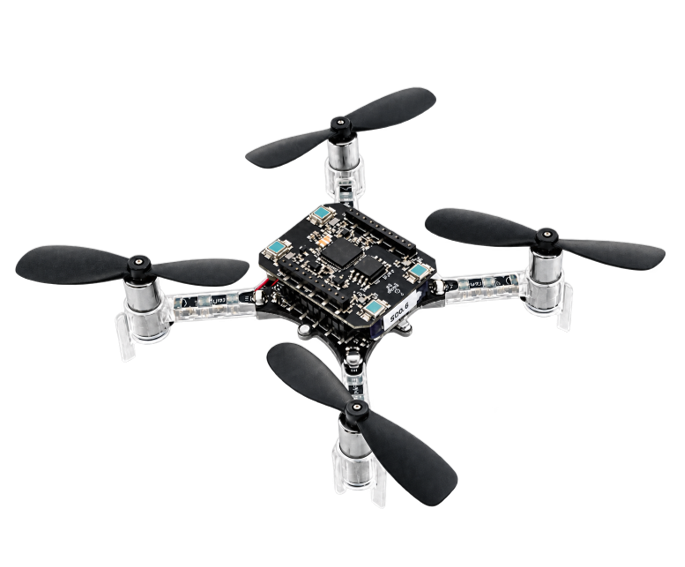
\includegraphics[height=3.08cm]{Methodology/Physical_Environment.png}};

\node[font=\bfseries\normalsize,align=center] (dtitle) at (9.0,7.70)
  {Digital twin ($\circ$)\\[-0.2mm]{\normalfont\normalsize Objective: improve model parameters $\theta_p^{(m)}$}};
\node (dimage) at (9.0,5.55)
  {
\includegraphics[height=3.08cm]{Methodology/Digital_Twin.png}};

% Physical environment
\node[block] (b1) at (0,2.75) {
  \textbf{Deployed policy $\pi_\bullet^{(n)}$}\\[1mm]
  $e_n=1$: information $\pi_\iota(\cdot\mid\theta_\iota^{(n)})$\\
  $e_n=0$: performance $\pi_\bullet(\cdot\mid\theta_\pi^{(n)})$
};

\node[block] (b2) at (0,0.35) {
  \textbf{Physical episode $n$}\\[1mm]
  hidden state $\mathbf{s}_\bullet$, input $\mathbf z$\\
  noisy observations $\mathbf{o}_\bullet$
};

\node[block] (b3) at (0,-2.10) {
  \textbf{Record $\mathcal E^{(n)}$}\\[1mm]
  $\mathcal E^{(n)}$ put in replay buffer $\mathcal B$;\\
  evaluated $\mathcal R_\bullet^{(n)}$
  
};

% Digital twin
\node[block] (b6) at (9.0,2.75) {
  \textbf{Choice of the next interaction}\\[1mm]
  $e_n=1$: $\mathcal J_{\mathrm{info}}\rightarrow\theta_\iota^{(n+1)}$
  \\
  $e_n=0$: $\widehat{\mathcal R}_\bullet(\mathcal R_\bullet,\mathcal R_\circ,\theta_\pi)$
  $\rightarrow\theta_\pi^{(n+1)}$
};

\node[block] (b5) at (9.0,0.35) {
  \textbf{Virtual candidate evaluation}\\[1mm]
  $e_n=1$: informativeness $\mathcal J_{\mathrm{info}}(\theta_\iota)$
  \\
  $e_n=0$: $\theta_p^{(m+1)}\rightarrow\theta_{\pi,\mathrm{MB}}$
};

\node[block] (b4) at (9.0,-2.10) {
  \textbf{Factual replay}\\[1mm]
  
  initial-state reconstruction\\
  $e_n=1$: $\mathbf o_\circ$ vs. $\mathbf o_\bullet\rightarrow\theta_p^{(m+1)}$ updated\\
  $e_n=0$: $\theta_p^{(m+1)}=\theta_p^{(m)}$
};

% Number labels
\node[number, anchor=center] at ([xshift=-3.08cm,yshift=0.78cm]b1.center) {1};
\node[number, anchor=center] at ([xshift=-3.08cm,yshift=0.78cm]b2.center) {2};
\node[number, anchor=center] at ([xshift=-3.08cm,yshift=0.78cm]b3.center) {3};
\node[number, anchor=center] at ([xshift=-3.08cm,yshift=0.78cm]b4.center) {4};
\node[number, anchor=center] at ([xshift=-3.08cm,yshift=0.78cm]b5.center) {5};
\node[number, anchor=center] at ([xshift=-3.08cm,yshift=0.78cm]b6.center) {6};

% Main loop
\draw[flow] (b1.south) -- node[note,right]{deploy} (b2.north);
\draw[flow] (b2.south) -- node[note,right]{measure} (b3.north);
\draw[flow] (b3.east) -- node[note,below]{replay buffer $\mathcal B$} (b4.west);
\draw[flow] (b4.north) -- node[note,right,text width=3.35cm,align=center]{
  $\theta_p^{(m+1)}$\\
  } (b5.south);
\draw[flow] (b5.north) -- node[note,right]{
  $\mathcal R_\circ,\,\theta_{\pi,\mathrm{MB}},\,\mathcal J_{\mathrm{info}}$} (b6.south);
\draw[flow] (b6.west) -- node[note,above,text width=3.2cm,align=center]{
  next interaction:\\[0.8mm] $\theta_\pi^{(n+1)}$ or $\theta_\iota^{(n+1)}$} (b1.east);

% Measured performance data bypasses factual identification
\draw[flow] (b3.east) -- ++(1.00,0) coordinate (retcorner)  -- node[note,rotate=90,above]{
  measured returns $(\theta_\pi^{(n)},\mathcal R_\bullet^{(n)})$} (retcorner |- b6.south west)  -- (b6.south west);

% Panel backgrounds
\begin{scope}[on background layer]
  \node[fit=(ptitle)(pimage)(b1)(b2)(b3),
        fill=black!5, draw=black!12, rounded corners=8pt,
        inner sep=10pt] {};
  \node[fit=(dtitle)(dimage)(b4)(b5)(b6),
        fill=white, draw=black!35, rounded corners=8pt,
        inner sep=10pt] {};
\end{scope}

\end{tikzpicture}%
}
\caption{Reinforcement Twinning closed-loop adopted in this work. The physical environment and its active Digital Twin evolve side by side through physical observations and virtual candidate evaluations, in order to achieve their respective objectives. The selector $e_n$ distinguishes information-oriented ($e_n=1$) and performance-oriented ($e_n=0$) interactions, keeping a common loop for both cases.}
\label{fig:rt_framework}
\end{figure*}
The actions carried out in each block can be summarized as follows:
\begin{enumerate}
    \item Policy deployment: the iteration starts from the parameters selected at the end of the previous DT evaluation. The first interaction uses the baseline policy $\pi_{\mathrm{BL}}$, executed through the built-in PID controller, and provides the reference performance for comparison with the optimized policies. For $e_n=1$, the deployed policy is an information-oriented policy $\pi_{\iota}(\cdot\mid\boldsymbol{\theta}_{\iota}^{(n)})$; for $e_n=0$, it is a performance-oriented policy $\pi_{\bullet}(\cdot\mid\boldsymbol{\theta}_{\pi}^{(n)})$. This first block converts a design decision made in the DT into an executable command for the physical controller. The policy representation, its admissible parameter set, and all safety checks are application dependent, but the RT principle is unchanged: the DT proposes the interaction, while the physical environment supplies the evidence that determines whether the proposal was useful.
    \item Physical episode: the physical environment evolves under its hidden dynamics, the deployed policy, and the exogenous input $\mathbf d$. The latter collects quantities that influence the episode without being selected by the policy, such as environmental disturbances, initial-condition variations, or changes in available actuation. The internal state $\mathbf s_{\bullet}$ is not generally known. RT receives the noisy observations $\mathbf o_{\bullet}$, the commanded inputs, and the operating conditions that are needed to reconstruct the episode. This distinction is essential because the DT is updated from what the experiment can actually measure.
    \item Recording: the observations, deployed policy, operating condition, control signals, exogenous inputs, and evaluated physical reward are collected in the episode record $\mathcal E^{(n)}$ and appended to the replay buffer $\mathcal B$. The purpose of this passage is to preserve a common, traceable description of the interaction before the information and performance branches use it differently. The replay buffer therefore links all later virtual operations to the experiment that produced their data and permits a model update to be repeated on the complete cumulative dataset.
    \item Factual replay: the DT reconstructs the initial state and replays the recorded policy under the measured operating conditions. When $e_n=1$, DT observations $\mathbf o_{\circ}$ are compared with $\mathbf o_{\bullet}$ and the mismatch is differentiated through the closed-loop twin. The model parameters are then updated from $\boldsymbol{\theta}_p^{(m)}$ to $\boldsymbol{\theta}_p^{(m+1)}$ using the cumulative replay buffer. When $e_n=0$, the model parameters remain frozen, so that $\boldsymbol{\theta}_p^{(m+1)}=\boldsymbol{\theta}_p^{(m)}$. The new policy-reward pair bypasses identification and instead augments the dataset used to learn the reward-transfer surrogate. Factual replay thus has a different learning target in the two phases, while the recorded evidence entering the loop remains the same.
    \item Virtual candidate evaluation: with the current model parameters, the DT evaluates interactions that have not yet been carried out. In the information branch, information-oriented policies are propagated through the closed-loop model, differentiated with respect to $\boldsymbol{\theta}_p$, and scored by the information they are expected to add to the weakest parameter direction. In the performance branch, the converged DT first provides the model-based policy $\pi_{\mathrm{MB}}$. Candidate deviations around this policy are then simulated, rejected if they violate the DT safety checks, and assigned both a DT reward and a reward-transfer surrogate prediction of their physical reward. This block is the main computational advantage of RT: a large candidate set can be explored in the DT while only a small number of selected policies reaches the physical environment.
    \item Choice of the next interaction: the final block converts the virtual evaluations into the next physical policy. For $e_n=1$, Eq.~\eqref{eq:rt-e-optimal} selects the candidate that maximizes the smallest eigenvalue of the cumulative Fisher matrix and therefore strengthens the least-observed joint parameter direction. For $e_n=0$, Eq.~\eqref{eq:rt-next-performance} selects the candidate with the largest Expected Improvement, balancing a high predicted physical reward against uncertainty in the learned transfer. The selected parameters are returned to Block~1, the physical episode index advances from $n$ to $n+1$, and the loop repeats. In the present work, the model-update index $m$ advances only in the information phase; separating the two indices makes clear that collecting a new performance episode does not imply a new model update.
\end{enumerate}

The selector value is scheduled within the test campaign. The loop first repeats Blocks~1-6 with $e_n=1$ until the model satisfies the adopted convergence and uncertainty criteria. It then switches once to $e_n=0$ and keeps the identified parameters fixed while the reward-transfer surrogate is refined. The following subsection specializes every element of this generic loop for the adopted test case.
\subsection{Test Case Physical and Digital Environments}
\label{sec:setup}
\paragraph*{Experimental setup}
The experiments are designed to reproduce a transition between out-of-ground-effect (OGE) and in-ground-effect (IGE) conditions over a finite obstacle while maintaining a constant forward flight speed. The experimental setup and adopted reference frame are illustrated in Fig.~\ref{fig:experimental_setup}.

The campaign is performed using a Crazyflie 2.1+ MAV from Bitcraze flying in the $x$-$z$ plane at $y=0$~m. The horizontal reference frame retains its origin at $x=y=0$, whereas the vertical origin is placed at the upper surface of the obstacle, so that $z=0$ at the obstacle height. Positive $z$ therefore measures the vertical distance of the vehicle from this surface, and $z/R$ is the corresponding nondimensional clearance, with $R=23$~mm. Each test begins at $x=0$~m, where the MAV reaches the prescribed altitude and hovers for 10~s. It then accelerates smoothly and reaches the desired forward speed around $x=1.0$-$1.2$~m while maintaining the prescribed $z/R$. The region of interest used for comparison with the DT results spans $x=1.70$-$4.00$~m. The MAV subsequently decelerates and lands around $x=4.20$~m. Within the region of interest, the obstacle extends from $x=2.20$~m to $x=3.01$~m, corresponding to a streamwise length of $0.81$~m. In the results, the streamwise coordinate is shifted to the beginning of the region of interest and normalized by $R$; consequently, this region covers $0\leq x/R\leq100$, while the obstacle occupies approximately $21.7\leq x/R\leq57.0$.

The Crazyflie 2.1+ is equipped with an onboard IMU sensor for attitude control and a Lighthouse positioning deck for position control. Together with a 350 mAh battery, the drone mass is around $m=32.42$~g. To provide a continuous position reference, the Lighthouse deck is detected by two Lighthouse infrared stations. Their placement is selected such that the MAV remains visible to at least one station throughout the complete trajectory. In the region directly above the obstacle, which constitutes the main area of interest for the GE experiments, the fields of view of the two stations intentionally overlap. This configuration reduces the probability of temporary tracking loss or a position-estimation disturbance caused by an interruption of the optical link between a Lighthouse station and the Lighthouse deck mounted on the Crazyflie. The Lighthouse positioning system provides sub-centimetre-level absolute accuracy and sub-millimetre repeatability. In flight experiments, Taffanel et al.~\cite{Taffanel2021Lighthouse} reported an average positioning error of approximately $0.5-1$~cm and an RMS position jitter between $0.5$ and $1$~mm, depending on the adopted estimator. 

\begin{figure*}[t]
    \centering
    \resizebox{0.98\textwidth}{!}{%
    \begin{tikzpicture}[>=Latex,font=\small]
        \path[use as bounding box] (-7.4,-2.15) rectangle (7.4,5.25);

        % Lighthouse fields of view
        \begin{scope}[on background layer]
            \clip (-7.4,-2.15) rectangle (7.4,5.25);
            \fill[red!18,opacity=0.16] (-6.25,3.95) -- (-8.00,-2.05) -- (23.00,-2.05) -- cycle;
            \fill[red!18,opacity=0.16] ( 6.25,3.95) -- ( 8.00,-2.05) -- (-23.00,-2.05) -- cycle;
        \end{scope}

        % Lighthouse stations; station 1 is mirrored from the same PNG
        \node (lh1) at (-6.25,4.15) {\reflectbox{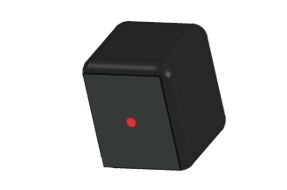
\includegraphics[width=1.45cm]{Setups/lighthouse.png}}};
        \node (lh2) at ( 6.25,4.15) {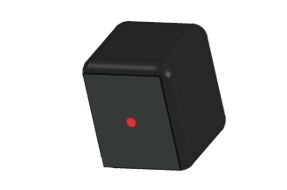
\includegraphics[width=1.45cm]{Setups/lighthouse.png}};
        \node[draw,rounded corners=2pt,fill=white,inner sep=3pt,anchor=south] at (-6.25,4.86) {Lighthouse station 1};
        \node[draw,rounded corners=2pt,fill=white,inner sep=3pt,anchor=south] at ( 6.25,4.86) {Lighthouse station 2};

        % Nominal crossing and repeated vehicle poses
        \draw[densely dashed,black!55,line width=0.8pt] (-5.45,1.55) -- (5.45,1.55);
        \node[green!45!black,font=\normalsize] at (-3.25,3.18) {$v_x^\ast/v_h\simeq\mathrm{const}$};
        \draw[->,very thick,green!45!black] (-3.90,2.88) -- (-2.60,2.88);
        \foreach \xx/\op in {-4.65/0.18,-2.45/0.34,-0.20/0.52,2.05/0.74,4.30/1.00}{
            \node[opacity=\op] at (\xx,1.62) {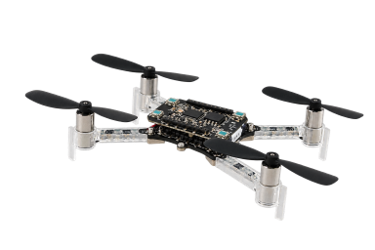
\includegraphics[width=2.20cm]{Setups/drone.png}};
        }
        \node[draw,rounded corners=2pt,fill=white,inner sep=3pt,align=center,anchor=south] at (0.85,2.38)
            {Crazyflie 2.1+ with Lighthouse deck};

        % Finite obstacle and vertical clearance
        \node[anchor=north] (obs) at (0,0.62) {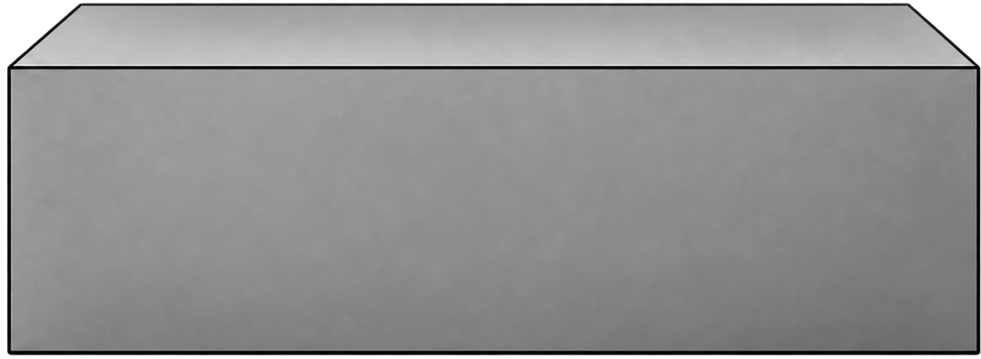
\includegraphics[width=6.60cm]{Setups/obstacle.png}};
        \node[draw,rounded corners=2pt,fill=white,inner sep=3pt] at (0,-1.45) {Finite obstacle};
        \draw[<->,very thick,red!75!black] (1.15,0.25) -- (1.15,1.55)
            node[midway,right] {$z^\ast/R$};

        % Useful optical volume and adopted reference frame
        \draw[densely dotted,green!45!black,line width=0.8pt] (-4.30,-1.88) -- (-4.30,3.00);
        \draw[densely dotted,green!45!black,line width=0.8pt] ( 6.10,-1.88) -- ( 6.10,3.00);
        \coordinate (O) at (-6.25,0.25);
        \fill (O) circle (1.4pt);
        \draw[->,thick] (O) -- ++(0.95,0) node[right] {$x$};
        \draw[->,thick] (O) -- ++(0,0.95) node[above] {$z$};
        \draw[->,thick] (O) -- ++(-0.58,-0.42) node[below left] {$y$};
    \end{tikzpicture}%
    }
    \caption{Experimental setup, operating trajectory, Lighthouse coverage, and adopted reference frame.}
    \label{fig:experimental_setup}
\end{figure*}

During each run, the Crazyflie firmware records the vehicle state, control response, and operating conditions. The logged quantities include position and translational velocity, attitude and angular rates, acceleration, battery voltage, collective-thrust command, and the individual motor PWM commands. The complete record is retained for trajectory assessment and for reconstructing each physical episode in the DT. For GE identification, the physical and DT trajectories are aligned along the streamwise coordinate, and the adjoint optimization minimizes the normalized vertical-position discrepancy over the obstacle region. The remaining channels support initialization and replay of the measured operating conditions, but do not enter the identification objective directly.

The Crazyflie is operated using its standard cascaded PID control architecture, as documented by Bitcraze~\cite{BitcrazeControllers}. An outer position loop tracks the desired position $\mathbf{x}^{*}$ and generates the corresponding velocity references $\mathbf{v}^{*}$. A velocity loop then regulates the translational motion, producing the desired roll and pitch angles together with the collective thrust command. These references are passed to the attitude controller, which determines the desired body angular rates. Finally, the inner angular-rate controller generates the roll, pitch, and yaw control contributions, which are combined with the collective thrust through the onboard motor mixer to determine the four individual motor commands. The same control architecture and firmware logic are reproduced in the DT from the official implementation~\cite{BitcrazeFirmware}, ensuring consistency between the numerical and experimental closed-loop dynamics.

\paragraph*{Digital Twin}
\label{sec:digital_twin}

The Digital Twin developed in this work follows the modeling formulation proposed by Richardson et al.~\cite{Richardson2025} for low-speed free flight and is tailored to reproduce the dynamics of the Crazyflie 2.1+ employed in the experimental campaign. The model is implemented as a differentiable physics-based simulator using the JAX library in Python and is used for both model identification and control optimization. The vehicle kinematics, rigid-body dynamics, propulsion system, battery dependence, actuator dynamics, and cascaded controller together form the nominal starting DT. Their parameters are inherited unchanged from Richardson et al.; they are neither reidentified nor independently revalidated in the present campaign. The finite-obstacle ground-effect correction is incorporated below as the unknown model component with associated $\boldsymbol{\theta}_p$ learned by RT.

The Crazyflie is modeled as a six-degree-of-freedom rigid body. Its state is described by position $\mathbf{x}=[x,y,z]^T$ and translational velocity $\mathbf{v}=[v_x,v_y,v_z]^T$ expressed in the inertial frame, the attitude quaternion $\mathbf{q}=[q_w,q_x,q_y,q_z]^T$, and the angular velocity $\boldsymbol{\omega}=[\omega_x,\omega_y,\omega_z]^T$ expressed in the body-fixed frame. The rotational speed of rotor $i$ is represented by $\Omega_i$.

The translational dynamics evaluated at the center of mass (CoM) are
%
\begin{equation}
\begin{cases}
{\dot{\mathbf{x}}=\mathbf{v}}\\
{m\dot{\mathbf{v}}=m\mathbf{g}+\mathbf{R}\mathbf{F}_{B}}
\end{cases}
\label{eq_vehicle_trasl}
\end{equation}
where $\mathbf{g}=[0,0,-g]^T$, $g$ is the gravitational acceleration, and $\mathbf{R}\in SO(3)$ transforms quantities from the body-fixed frame to the inertial frame. The total force in body coordinates is $\mathbf{F}_{B}=[0,0,T]^T$, where $T$ is the total thrust generated by the four rotors.
%

The rotational dynamics follow Euler's rigid-body equation,
%
\begin{equation}
\mathbf{I}\dot{\boldsymbol{\omega}}
+
\boldsymbol{\omega}
\times
(\mathbf{I}\boldsymbol{\omega})
= \boldsymbol{\tau}
\label{eq_vehicle_rot}
\end{equation}
where $\mathbf{I}$ is the inertia tensor and $\boldsymbol{\tau}=[\tau_x,\tau_y,\tau_z]^T$ is the total moment vector expressed in body coordinates.
%
The vehicle attitude is propagated through the unit quaternion according to
%
\begin{equation}
\dot{\mathbf q} = \frac{1}{2}
\mathbf{\Lambda}(\boldsymbol{\omega})\mathbf q
\label{eq_vehicle_attitude}
\end{equation}
where $\mathbf{\Lambda}(\boldsymbol{\omega})$ is the scalar-first quaternion kinematic matrix associated with the body angular velocity, using the convention adopted by Richardson et al.~\cite{Richardson2025}.
%
The thrust and reaction torque generated by rotor $i$ are modeled as
%
\begin{equation}
\begin{cases}
{T_i=k_T\Omega_i^2}\\
{Q_i=k_Q\Omega_i^2}
\end{cases}
\label{eq_T_and_Q}
\end{equation}
where $T_i$ and $Q_i$ are the individual rotor thrust and torque and $k_T$ and $k_Q$ are the corresponding coefficients. The total thrust and moments follow from their signed combination.
%
For the adopted quadcopter and motor convention, the roll ($\tau_R$), pitch ($\tau_P$), and yaw ($\tau_Y$) moments are
%
\begin{equation}
\begin{cases}
{\tau_R=
\frac{d}{2}
\left(
-T_1-T_2+T_3+T_4
\right)}\\
{\tau_P=
\frac{d}{2}
\left(
-T_1+T_2+T_3-T_4
\right)}\\
{\tau_Y=
\sum_{i=1}^{4}s_iQ_i,}
\end{cases}
\label{eq_RP_moments}
\end{equation}
where $d$ is the motor-to-motor distance and $s_i\in\{-1,+1\}$ identifies the rotation direction of rotor $i$.
%

The connection between the motor commands and propeller speed follows the Crazyflie propulsion characterization adopted by Richardson et al. The effect of battery state is included through the battery voltage $V_b=f(\mathrm{SOC})$, where $\mathrm{SOC}$ denotes the battery state of charge. A voltage correction factor is defined as $\eta_V=V_b/V_{\mathrm{ref}}$, where $V_{\mathrm{ref}}$ is the voltage of a fully charged battery. The rotor-speed command associated with the PWM input is corrected as $\Omega_{\mathrm{cmd}}=\eta_V\Omega_{\mathrm{PWM}}$. The realized rotor speed follows this command through a first-order actuator model with time constant $\tau_{\mathrm{rpm}}=0.020$~s. This value is inherited from the Richardson model and is not identified in the present work.

The main physical parameters adopted in the DT are taken from the formulation of \cite{Richardson2025} and are summarized in Table~\ref{tab:dt_parameters}. The nominal propulsion model retains the battery-voltage correction $V_b=f(\mathrm{SOC})$. However, both physical and DT missions start with a fully charged battery and last only a few seconds; therefore, the within-mission change of state of charge is neglected. The vehicle dynamics are coupled with the same cascaded PID architecture used in the physical environment, providing the nominal closed-loop model on which the ground-effect correction is identified.
\begin{table}[t]
\centering
\caption{Baseline DT parameters adopted from Richardson et al.~\cite{Richardson2025}.}
\label{tab:dt_parameters}
\begin{tabular}{lc}
\hline
Parameter & Value \\
\hline
$m$ & $0.03242$ kg\\
$R$ & $0.023$ m \\
$d$ & $0.065$ m \\
$I_{xx}$ & $16.57\times10^{-6}$ kg m$^2$ \\
$I_{yy}$ & $16.56\times10^{-6}$ kg m$^2$ \\
$I_{zz}$ & $29.26\times10^{-6}$ kg m$^2$ \\
$k_T$ & $2.88\times10^{-8}$ N s$^2$/rad$^2$ \\
$k_Q$ & $7.24\times10^{-10}$ N m s$^2$/rad$^2$ \\
$\tau_{\mathrm{rpm}}$ & $0.020$ s \\
$V_{\mathrm{ref}}$ & $4.20$ V \\
\hline
\end{tabular}
\end{table}
\paragraph*{Ground-effect correction}
\label{sec:ge-model}
The described nominal DT reproduces the vehicle dynamics in free flight and was validated in those conditions by Richardson et al.~\cite{Richardson2025}. The nominal DT, however,  does not account for the additional rotor-surface interaction generated as the vehicle closely crosses the finite obstacle. This interaction is introduced through a deliberately simple physical model inspired by the analytical formulation of Cheeseman and Bennett for an isolated rotor in hovering~\cite{CheesemanBennett1955}. For a rotor $i$ of radius $R$ at a clearance $z_i$ from the obstacle, the in-ground-effect thrust $T_{i,\mathrm{IGE}}$ is obtained from the nominal out-of-ground-effect thrust $T_{i,\mathrm{OGE}}$ through the amplification factor $f_{\mathrm{GE}}$,
\begin{equation}
 T_{i,\mathrm{IGE}}
 =T_{i,\mathrm{OGE}}\,
 f_{\mathrm{GE}}(z_i;\boldsymbol{\theta}_p).
 \label{eq:ge-thrust-factor}
\end{equation}
The amplification factor is modeled as
\begin{equation}
 f_{\mathrm{GE}}(z_i;\boldsymbol{\theta}_p)=1+A\left(\frac{R}{z_i}\right)^p,
 \qquad \boldsymbol{\theta}_p=[A,\,p]^\top .
 \label{eq:fge}
\end{equation}
Here, $A$ controls the magnitude of the thrust augmentation, while $p$ determines how rapidly the interaction decays with increasing clearance. The original Cheeseman and Bennett formulation rearranged with the same unknowns would have retained $A=1/16$ and $p=2$. These values initialize the identification in the present work, while both coefficients remain free to adapt to the present vehicle and operating conditions.

This model is deliberately low order: ground effect is treated as a static function of the instantaneous rotor clearance. Measurements by Kan et al.~\cite{Kan2019} indicate that velocity dependence is limited over the low-speed range considered here, but it is not assumed to vanish. The formulation also omits the transient development and decay of the rotor-surface interaction as the vehicle crosses the obstacle edges. These omissions preserve a compact model that can be identified and differentiated efficiently, while leaving a structural discrepancy that is addressed later through the reward-transfer surrogate.

Equation~\eqref{eq:fge} describes the clearance dependence above an extended surface. The obstacle considered here occupies only a finite streamwise interval, so the augmentation must also depend on the position of each rotor relative to its edges. It is therefore weighted by $\chi_i(x)\in[0,1]$, defined as the fraction of rotor disk $i$ that overlaps the obstacle. The corrected rotor thrust becomes
\begin{equation}
 T_{i,\mathrm{corr}}=T_{i,\mathrm{OGE}}\left[1+\chi_i(x)\left(f_{\mathrm{GE}}(z_i;\boldsymbol{\theta}_p)-1\right)\right],
 \label{eq:corrected-thrust}
\end{equation}
where $T_{i,\mathrm{OGE}}$ is the nominal rotor thrust outside ground effect. The overlap fraction is zero when the rotor lies outside the obstacle footprint and reaches unity when its disk is fully above it. Its continuous variation across the leading and trailing edges avoids discontinuous force changes and naturally accounts for the four rotors entering and leaving the obstacle region at different streamwise positions. 

\subsection{Test Campaign Overview}
\label{sec:test-campaign}
Following Kan et al.~\cite{Kan2019}, the desired forward velocity is normalized by the ideal induced velocity in hover,
\begin{equation}
 v_h=\sqrt{\frac{T_{h,r}}{2\rho_a\pi R^2}}
 =\sqrt{\frac{mg}{8\rho_a\pi R^2}},
 \label{eq:hover-induced-velocity}
\end{equation}
where $T_{h,r}=mg/4$ is the hover thrust required from each rotor, $\rho_a$ is the air density, and $R$ is the rotor radius. With $m=32.42$~g, $R=0.023$~m, and $\rho_a=1.225$~kg/m$^3$, Eq.~\eqref{eq:hover-induced-velocity} gives $v_h\simeq4.42$~m/s. An operating condition is henceforth denoted by the ordered pair $(z^\ast/R,\,v_x^\ast/v_h)$.

The test campaign follows the sequential RT schedule introduced above. All tests use the same physical environment, DT structure, reference frame, and data-processing procedure described in Sec.~\ref{sec:setup}. The nominal operating condition is $(z^\ast/R,\,v_x^\ast/v_h)=(1.5,0.079)$. Unless stated otherwise, policy design, model identification, and reward evaluation refer to this condition. The campaign is organized into five consecutive blocks, introduced below together with the notation used in the results.

\paragraph*{\textit{Baseline policy}}
The campaign starts from the built-in cascaded PID controller at the nominal condition $(z^\ast/R,\,v_x^\ast/v_h)=(1.5,0.079)$. This policy is denoted by $\pi_{\mathrm{BL}}$ and is repeated experimentally to quantify run-to-run variability. Its mean response and RMS band provide the reference trajectory statistics, the first record in the replay buffer, and the baseline tracking cost used to normalize the rewards reported later. Since $\pi_{\mathrm{BL}}$ reacts only after the vehicle departs from the desired clearance, it also exposes the ground-effect excursion that the subsequent predictive policies are designed to anticipate.

\paragraph*{\textit{Information phase}}
\label{sec:information-phase}
The objective of the information phase is to design and perform trajectories that improve the identification of the unknown parameters $\boldsymbol{\theta}_p=[A,p]$ of the ground-effect model described by Eqs.~\eqref{eq:ge-thrust-factor} and~\eqref{eq:fge}.
Each trajectory deployed in the physical environment is replayed through the differentiable DT with the same reference and reconstructed initial condition used experimentally. Factual replay identifies the coefficient pair from the accumulated tracking response. The subsequent DT design searches for a safe altitude reference that adds information along the least-observed parameter direction, thereby defining the next experiment. The two operations are repeated sequentially, with each new flight updating both the identified parameters and the information available for the next design.

The model is initialized from the Cheeseman-Bennett coefficients, $A=1/16$ and $p=2$. Starting from the baseline record, twelve information-oriented policies $\pi_{\mathrm{INF}}^{(n)}$ are added sequentially to the cumulative dataset. The first six policies are designed over the broad admissible clearance range $0.5<z/R<6$. This first stage deliberately explores a wide set of altitude histories: it establishes the global scale and decay of the interaction without assuming in advance that the most useful data must come from the smallest admissible clearance, and it verifies the response of the evolving DT over the complete safe operating range.

By the end of the sixth information-oriented episode, new policies in the broad domain still increase the cumulative Fisher information, but their marginal E-optimal contribution has become modest compared with the first information-oriented interaction. This behavior is physically consistent with Eq.~\eqref{eq:fge}: at larger clearances, $f_{\mathrm{GE}}$ approaches unity and its sensitivity to both $A$ and $p$ decreases. The admissible design domain is therefore restricted to $0.5<z/R<1.5$ for the remaining six policies, defining the near-wall domain. The restriction is an adaptive design decision, not a rejection of the broad-domain data. All preceding episodes remain in the replay buffer, while the new candidates concentrate the available experimental effort where the identified law is steepest and the weak parameter direction can be excited more effectively. After every flight, the new record is appended to the cumulative dataset and the identification is warm-started from the preceding converged coefficients.

The information phase begins with factual replay and adjoint identification. For physical episode $n$, the experimental record provides the measured altitude-tracking error, the deployed reference policy, and the reconstructed initial condition. The DT replays the same episode with the current model parameters $\boldsymbol{\theta}_p$. The experimental and virtual error histories are evaluated at the same $K_n$ spatial positions encountered during the flight and collected in the vectors
\begin{align}
 \mathbf e_{z,n}^{\bullet}
 &=\bigl[e_{z,n}^{\bullet}(x_{n,1}),\ldots,
 e_{z,n}^{\bullet}(x_{n,K_n})\bigr]^{\mathsf T},\\
 \mathbf e_{z,n}^{\circ}(\boldsymbol{\theta}_p)
 &=\bigl[e_{z,n}^{\circ}(x_{n,1};\boldsymbol{\theta}_p),\ldots,
 e_{z,n}^{\circ}(x_{n,K_n};\boldsymbol{\theta}_p)\bigr]^{\mathsf T}.
 \label{eq:episode-error-vectors}
\end{align}
With $N$ episodes in the replay buffer, the identification loss is
\begin{equation}
 J_p(\boldsymbol{\theta}_p)=
 \frac{1}{N}\sum_{n=1}^{N}
 \frac{1}{K_n}
 \left\|
 \frac{\mathbf e_{z,n}^{\circ}(\boldsymbol{\theta}_p)
       -\mathbf e_{z,n}^{\bullet}}{R}
 \right\|_2^2.
 \label{eq:identification-loss}
\end{equation}
The factor $1/K_n$ gives every episode equal weight irrespective of its number of samples or duration.

The loss is minimized by differentiating the complete time-discrete closed-loop rollout in reverse mode. This is the discrete-adjoint formulation of the identification problem: the loss sensitivity is propagated backward through the vehicle dynamics, actuator model, controller states, and ground-effect correction. At optimization step $t$, the resulting gradient is
\begin{equation}
 \mathbf{g}_t=
 \nabla_{\boldsymbol{\theta}_p}J_p
 \bigl(\boldsymbol{\theta}_{p,t}\bigr)
 =
 \begin{bmatrix}
 \dfrac{\partial J_p}{\partial A} &
 \dfrac{\partial J_p}{\partial p}
 \end{bmatrix}^{\mathsf T}.
 \label{eq:adjoint-gradient}
\end{equation}
It accounts for the direct influence of $A$ and $p$ on the aerodynamic forces and for the trajectory changes produced through the closed feedback loop. Both derivatives are obtained in one backward pass, without a separate perturbed simulation for each parameter.

Adam uses this gradient to update the parameters over successive optimization steps. It retains a first moment $\mathbf{m}_t$, which smooths the gradient direction, and a second moment $\mathbf{v}_t$, which tracks its component-wise squared magnitude:
\begin{align}
 \mathbf{m}_t &=
 \beta_1\mathbf{m}_{t-1}
 +(1-\beta_1)\mathbf{g}_t,\\
 \mathbf{v}_t &=
 \beta_2\mathbf{v}_{t-1}
 +(1-\beta_2)\mathbf{g}_t^{\odot 2}.
 \label{eq:adam-moments}
\end{align}
The two moments allow the step size to adapt separately to $A$ and $p$, whose gradients can have different scales. After the standard bias correction, the next parameter vector is
\begin{equation}
 \boldsymbol{\theta}_{p,t+1}=
 \Pi_{\Theta}\!\left[
 \boldsymbol{\theta}_{p,t}
 -\eta
 \frac{\widehat{\mathbf{m}}_t}
 {\sqrt{\widehat{\mathbf{v}}_t}+\epsilon}
 \right],
 \label{eq:adjoint-adam}
\end{equation}
where $\eta$ is the chosen learning rate, $\epsilon$ prevents division by zero, and $\Pi_{\Theta}$ keeps the solution inside the physically admissible set $\Theta$. In the present campaign, $\eta=5\times10^{-3}$ and convergence is assessed over windows of 25 optimization steps. The relative-loss, coefficient-range, and projected-gradient tolerances are $2\times10^{-4}$, $10^{-3}$, and $5\times10^{-3}$, respectively. The optimization is considered converged only when all three conditions remain satisfied over a complete monitoring window. When a new physical episode is added, the next fit is warm-started from the previously converged parameters, while the Adam moments are reset because the cumulative objective has changed.

The converged estimate $\widehat{\boldsymbol{\theta}}_p$ is then used to determine which experiment should be performed next. Local parameter uncertainty is approximated from the curvature of the identification loss. Let
\begin{equation}
 \mathbf H=\nabla^2J_p(\widehat{\boldsymbol{\theta}}_p)
 =\mathbf Q\operatorname{diag}(\lambda_1,\lambda_2)\mathbf Q^{\mathsf T}.
\end{equation}
To avoid a singular inverse along a locally flat direction, the eigenvalues are floored at $\lambda_H=10^{-6}$. The resulting local inverse-Hessian approximation is
\begin{equation}
 \boldsymbol{\Sigma}_{\theta}\simeq
 \max\!\left[J_p(\widehat{\boldsymbol{\theta}}_p),10^{-12}\right]
 \mathbf Q\operatorname{diag}\!\left[
 \max(\lambda_1,\lambda_H)^{-1},
 \max(\lambda_2,\lambda_H)^{-1}
 \right]\mathbf Q^{\mathsf T}.
 \label{eq:parameter-covariance}
\end{equation}
This matrix is used as a local curvature-based uncertainty approximation, not as a calibrated finite-sample confidence region. A flat direction of the loss produces a larger local uncertainty. For a model output $g(\boldsymbol{\theta}_p)$, such as $f_{\mathrm{GE}}$ at a prescribed clearance, the corresponding linearized uncertainty indicator is
\begin{equation}
 \sigma_g^2=
 \nabla_{\boldsymbol{\theta}_p}g^{\mathsf T}
 \boldsymbol{\Sigma}_{\theta}
 \nabla_{\boldsymbol{\theta}_p}g.
 \label{eq:uncertainty-propagation}
\end{equation}
Thus, $A$ and $p$ may retain a strongly elongated and correlated local uncertainty region even when the resulting ground-effect curve is tightly constrained. The quantity $2\sigma_{f_{\mathrm{GE}}}/f_{\mathrm{GE}}$ reported later is the propagated relative uncertainty of the total thrust factor. It is not interpreted as an exact 95\% confidence interval, and its decrease at large clearance partly reflects that $f_{\mathrm{GE}}\rightarrow1$.

Candidate altitude-reference policies are then generated inside the admissible design space and simulated with the converged DT. Because $A$ and $p$ have different numerical scales, the sensitivity columns are normalized with the local parameter scales
\begin{equation}
 \mathbf D_{\theta}=\operatorname{diag}
 \left(\sqrt{[\boldsymbol{\Sigma}_{\theta}]_{AA}},
       \sqrt{[\boldsymbol{\Sigma}_{\theta}]_{pp}}\right),
 \qquad
 \overline{\mathbf S}_n=
 \frac{\partial\mathbf e_{z,n}^{\circ}}
 {\partial\boldsymbol{\theta}_p}\mathbf D_{\theta}.
\end{equation}
The eigenvalues can therefore be interpreted for perturbations of one local parameter standard deviation, rather than being dominated by the raw numerical scale of either coefficient. Under an independent, homoscedastic residual approximation, a common normalized residual variance is estimated as $\sigma_e^2=\max[J_p(\widehat{\boldsymbol{\theta}}_p),10^{-12}]$. The Fisher-information proxy accumulated from the $N$ completed experiments is
\begin{equation}
 \mathbf F_{1:N}=
 \sum_{n=1}^{N}
 \frac{\overline{\mathbf S}_n^{\mathsf T}\overline{\mathbf S}_n}
 {K_n\sigma_e^2},
 \label{eq:cumulative-fisher}
\end{equation}
where $K_n$ prevents a longer episode from appearing more informative solely because it contains more samples. Large eigenvalues of $\mathbf F_{1:N}$ correspond to locally scaled parameter combinations that the accumulated experiments constrain strongly; its smallest eigenvalue describes the least-observed joint parameter direction. Since spatial residuals can remain correlated, this matrix is used as a comparative design metric rather than as an exact statistical Fisher matrix. During sequential design it is evaluated with the current converged DT. For the post-campaign comparison reported later, every episode and the repeated-baseline counterfactual are reevaluated using the final DT, final parameter scaling, and the same residual variance, so their cumulative values are directly comparable.

Each virtual candidate policy $\pi$ produces a predicted Fisher contribution $\mathbf F(\pi)$. The next information-oriented policy is selected with the E-optimal criterion
\begin{equation}
 \pi_{\mathrm{INF}}^{(N+1)}=
 \arg\max_{\pi\in\Pi_{\mathrm{safe}}}
 \lambda_{\min}\!\left(
 \mathbf F_{1:N}+\mathbf F(\pi)
 \right),
 \label{eq:e-optimal-design}
\end{equation}
which selects the safe candidate predicted to increase the Fisher information along its weakest direction. The criterion already favors sensitivities that complement the accumulated dataset. A separate novelty check may nevertheless select a slightly less informative candidate when its predicted response is sufficiently different from the experiments already performed. Candidates that violate state, reference-rate, acceleration, actuator, or clearance constraints are discarded before deployment.

After the selected flight, its record is added to the replay buffer and the adjoint-Adam identification is repeated. The inner Adam loop is stopped by the numerical convergence conditions defined above. The complete information phase is terminated only when adding new episodes no longer changes the converged values of $A$ and $p$ appreciably and no longer produces a meaningful reduction in the magnitude of their estimated correlation.

\paragraph*{\textit{Model-based policy}}
\label{sec:mb-optimum}
After identification, $A$ and $p$ are frozen and the specialized performance loop uses the converged DT to improve altitude tracking across the finite obstacle. The control policy is implemented as a spatial reference governor above the unchanged cascaded PID controller, so the computationally expensive prediction and optimization remain offline while the deployed policy is a lightweight lookup table. First the DT produces the model-based policy $\pi_{\mathrm{MB}}$; physical rewards around that policy then train the reward-transfer surrogate used by Expected Improvement to design improved policies. The policy is the spatial altitude reference supplied to the governor,
\begin{equation}
 z_{\pi}(x)=z_{\mathrm{BL}}(x)+\Delta z_{\pi}(x),
 \label{eq:policy}
\end{equation}
where $z_{\mathrm{BL}}$ is the nominal mission reference altitude which is constant along $x$. The governor modifies only the vertical set point as a function of measured longitudinal position. The horizontal trajectory, attitude stabilization, motor mixing, and onboard PID gains remain unchanged. This spatial representation is preferred over the time representation as it prevents small DT-experiment timing differences from desynchronizing the anticipatory command from the obstacle.

At the nominal operating condition, the reference correction is parameterized at control points separated by one rotor radius, $\Delta x=R$, over the complete crossing and interpolated between consecutive points. Its amplitude is bounded by $|\Delta z|\leq3R$, while the predicted lowest rotor must retain a clearance of at least $0.5R$ from the local surface.

The model-based policy is first obtained through model-predictive reference synthesis.
The model-based policy $\pi_{\mathrm{MB}}$ is obtained from a finite-horizon nonlinear prediction of the complete closed-loop mission. At every optimizer step, the DT propagates the vehicle, propulsion, aerodynamic model, PID states, and reference governor over the entire prediction interval. Reverse-mode differentiation supplies the gradient with respect to all spatial reference values, and Adam updates their amplitudes subject to bound and endpoint projections. The optimized policy is therefore computed before the flight and then executed online as a lightweight interpolation table. In this work, \emph{model predictive control} refers to this model-predictive reference synthesis; a receding-horizon optimizer is not run onboard.

Performance is evaluated against the original mission reference used by the nominal cascaded PID controller. The tracking cost and corresponding reward are
\begin{equation}
 J_{\mathrm{trk}}(\pi)=\frac{1}{N_{\mathcal R}}
 \sum_{x_k\in\Omega_{\mathcal R}}
 \left[\frac{z_k-z_{\mathrm{BL}}(x_k)}{R}\right]^2,
 \qquad
 \mathcal{R}(\pi)=1-J_{\mathrm{trk}}(\pi).
 \label{eq:reward}
\end{equation}
The reported policy is optimized with the single final identified DT; no model-uncertainty ensemble is used. The objective augments the tracking term with amplitude, curvature, and clearance penalties,
\begin{align}
 J_{\mathrm{MB}}=&\;J_{\mathrm{trk}}
 +0.10\left\|\frac{\Delta z_{\pi}}{R}\right\|_2^2
 +2.0\left\|\mathbf{D}^2\frac{\Delta z_{\pi}}{R}\right\|_2^2 \notag\\
 &+10^5\Phi_{\mathrm{clr}}(\pi),
 \label{eq:mb-objective}
\end{align}
where $\mathbf{D}^2$ is the spatial second-difference operator and $\Phi_{\mathrm{clr}}$ is the mean squared violation of the $0.5R$ minimum clearance of the lowest rotor while it is above the obstacle. The amplitude term limits control authority, the curvature term suppresses spatially sharp commands, and the clearance term enforces safety on the tilted rotor geometry rather than only on the vehicle center of mass. The final policy is replayed once more in the DT and rejected if the hard clearance check fails.

\paragraph*{\textit{Performance phase}}
\label{sec:performance-phase}
The performance search is conducted at the nominal operating condition with the identified parameters frozen. Two interpolation policies, denoted collectively by $\pi_{\lambda,i}$ with $\lambda\in\{1/3,2/3\}$, are first tested between $\pi_{\mathrm{BL}}$ and $\pi_{\mathrm{MB}}$ to establish the global relation between the DT and physical rewards. The search is then expanded around $\pi_{\mathrm{MB}}$ using three smooth spatial basis functions. A scrambled Sobol library of 2000 coefficient vectors is screened in the DT, and seven admissible, mutually distinct policies $\pi_{\mathbf a,i}$ are deployed to train the local GP discrepancy. Subsequent policies $\pi_{\mathrm{EI},i}$ are selected sequentially by Expected Improvement; after each flight, the physical reward is appended to the reward-transfer surrogate dataset. The policy with the largest nominal-condition physical reward is denoted by $\pi_{\mathrm{EI}}^{\star}$.

Physical rewards are then used to refine this model-based policy and compensate for the remaining model discrepancy. Reinforcement Twinning uses these measurements to correct the local policy ranking predicted by the DT. A new candidate is written as
\begin{equation}
 \Delta z_{\pi}(x)=\Delta z_{\mathrm{MB}}(x)+
 R\,\mathbf{b}^{\mathsf T}(x)\mathbf a,
 \label{eq:rt-policy}
\end{equation}
where the smooth basis functions $\mathbf{b}(x)$ span the control-relevant portions of the mission and $\mathbf a=[a_A,a_B,a_C]^\top$ is the bounded vector of policy-modification coefficients. A space-filling library is first evaluated in the DT; the same reference and rotor-clearance checks used for the MB solution define the admissible set $\mathcal A_{\mathrm{safe}}$.

The affine component of the reward-transfer surrogate is fitted by ordinary least squares to the paired DT and physical rewards. The residual is modeled by a zero-mean Mat\'ern-$3/2$ GP. At the nominal operating condition, its input is the three-component vector $\mathbf a$, with each coordinate scaled by $0.30R$. The signal variance is initialized from the empirical variance of the affine residuals and is bounded below by $0.05^2$. The rewards are computed from the cleaned mean trajectories and are treated as deterministic campaign observations; a diagonal jitter of $10^{-8}$ is added only for numerical stability. Accordingly, the GP posterior standard deviation quantifies interpolation uncertainty within this surrogate and not run-to-run experimental dispersion. The resulting relation is
\begin{equation}
 \mathcal{R}_{\bullet}=
 \gamma_0+\gamma_1\mathcal{R}_{\circ}
 +\delta(\mathbf a,\boldsymbol{\chi})+\varepsilon,
 \label{eq:reward-transfer}
\end{equation}
where $\delta$ is the GP discrepancy and $\boldsymbol{\chi}$ contains optional operating conditions expressed by $(z^\ast/R,\,v_x^\ast/v_h)$. Two policies with similar DT performance can receive different physical corrections. Its posterior mean and variance are updated after every performance-oriented episode. Expected Improvement is used with zero exploration margin, $\xi=0$, and selects the next experiment,
\begin{align}
 Z(\mathbf a)&=
 \frac{\mu_{\bullet}(\mathbf a)-\mathcal{R}_{\bullet}^{+}}
 {\sigma_{\bullet}(\mathbf a)},\\
 \operatorname{EI}(\mathbf a)&=
 \left(\mu_{\bullet}-\mathcal{R}_{\bullet}^{+}\right)\Phi(Z)
 +\sigma_{\bullet}\phi(Z),\\
 \mathbf a_{n+1}&=
 \arg\max_{\mathbf a\in\mathcal A_{\mathrm{safe}}}
 \operatorname{EI}(\mathbf a),
 \label{eq:ei}
\end{align}
with zero improvement assigned to a vanishing posterior variance. The first term exploits candidates with a high predicted physical reward, whereas the second rewards unresolved but potentially useful regions. The model-based policy remains the reference throughout the search; data are used to learn the GP discrepancy that affects physical performance.

For transfer across operating conditions, the DT and physical performance are normalized by the corresponding condition-specific baseline cost,
\begin{equation}
 \mathcal S=1-\frac{J_{\pi}}{J_{\mathrm{BL}}}
   =1-\frac{1-\mathcal R_{\pi}}{1-\mathcal R_{\mathrm{BL}}},
 \label{eq:normalized-score}
\end{equation}
and $\boldsymbol{\chi}$ is augmented with the operating condition. Policy coordinates are defined relative to the local MB deformation. Consequently, a correction learned where the model-based action is large is reduced automatically when the local MB solution requires little intervention, rather than being transferred as a fixed altitude offset.

\paragraph*{\textit{Generalization}}
The final block evaluates whether the policy structure learned at the nominal condition remains useful when the operating condition changes. Two off-nominal conditions are considered: $(z^\ast/R,\,v_x^\ast/v_h)=(2.5,0.045)$ and $(1,0.113)$. For each condition, a baseline policy $\pi_{\mathrm{BL}}$ and a model-based policy $\pi_{\mathrm{MB}}$ are computed with the frozen identified DT. The best nominal RT correction is then transferred in the coordinates of the condition-specific model-based reference correction and denoted by $\pi_{\mathrm{EI}}^{\mathrm{tr}}$. Where an additional condition-specific EI search is performed, its best physical policy is denoted by $\pi_{\mathrm{EI}}^{\star}$. These tests distinguish direct transfer of the nominal correction from a local, proof-of-concept extension of the RT search at a new operating condition; they do not constitute convergence of a surrogate over the full velocity-clearance domain.


\section{Results and Discussion}
\label{sec:results}

\subsection{Baseline Response}
\label{sec:results-bl}

The first experimental case employs only the cascaded PID controller available in the original Crazyflie firmware. The most direct target for this baseline crossing is a constant-clearance trajectory at $(z^\ast/R,\,v_x^\ast/v_h)=(1.5,0.079)$. The desired trajectory is therefore the straight horizontal line denoted by $\pi_{\mathrm{BL}}$ and reported with a dashed line in Fig.~\ref{fig:stage0}. This case establishes the performance baseline because the controller acts exclusively through feedback, without any anticipation of the approaching aerodynamic interaction.

The solid line in Fig.~\ref{fig:stage0} reports the mean experimental trajectory $\mathrm{EXP}_{\mathrm{BL}}$ obtained from five repetitions, while the surrounding shaded region represents the corresponding $\pm\mathrm{RMS}$ run-to-run dispersion. At each streamwise position, this quantity is defined as $\mathrm{RMS}(x)=[N_r^{-1}\sum_{j=1}^{N_r}(z_j(x)-\overline z(x))^2]^{1/2}$, with $N_r=5$. The band therefore describes repeatability about the measured mean and is not an uncertainty interval for that mean. Before reaching the obstacle, the vehicle maintains an almost constant clearance close to the commanded value, supporting satisfactory tracking at this modest forward speed away from the surface interaction. The response changes markedly over the obstacle: the vehicle initially rises to approximately $z/R=2.5$ and subsequently settles around $z/R=2$. The additional thrust generated in ground effect produces the initial overshoot. The feedback controller reacts by reducing the motor speeds and commanded thrust, but this corrective action is insufficient to recover $z^*/R=1.5$ while the vehicle remains over the obstacle. The cascaded PID is tuned around hovering and contains no model that can anticipate the surface-induced thrust augmentation.

The opposite transient occurs at the trailing edge. Ground-effect augmentation disappears while the motor command is still reduced by the preceding feedback action, producing an undershoot down to approximately $z/R=0.5$. The vehicle then gradually recovers the commanded clearance, which is reached only about $40R$ downstream of the obstacle. Both excursions are substantially larger than the run-to-run dispersion, indicating a repeatable interaction rather than experimental scatter. The baseline experiment consequently provides the reference cost for all subsequent performance comparisons and the first factual record used during the information phase.

\begin{figure}[t]
\centering
\resultfigure{Results/stage_0_pid_baseline.pdf}
\caption{Baseline policy $\pi_{\mathrm{BL}}$ and mean experimental response $\mathrm{EXP}_{\mathrm{BL}}$ over five repetitions. The shaded band represents the corresponding $\pm\mathrm{RMS}$ dispersion.}
\label{fig:stage0}
\end{figure}

\subsection{Information Phase}
\label{sec:results-inf}

Each information-oriented policy is constructed by fixing a set of longitudinal nodes and allowing the optimizer to modify the local vertical reference at those nodes. Interpolation between consecutive values produces the continuous reference $z_{\pi}(x)$ deployed through the onboard PID controller. The longitudinal locations remain fixed, while the optimized nodal heights determine which clearances and altitude variations are requested during the crossing. The bounds of the design domain apply to this reference, not to the DT or physical vehicle trajectory, which can depart from it under the closed-loop dynamics.

Two consecutive design domains are used. The first six policies are generated in the \emph{broad domain}, with the reference bounded within $0.5<z/R<6$, allowing the optimizer to explore a broad range of vertical excitations. After these six policies, the upper bound is reduced to $z/R=1.5$ for the remaining six episodes, defining the \emph{near-wall domain}. The purpose of this restriction is to add information near the wall, where the ground-effect response is expected to be strongest and most sensitive to $A$ and $p$. Representative references and physical responses from both domains are reported in Fig.~\ref{fig:informative-policies}. The broad-domain policies $\pi_{\mathrm{INF},1}$ and $\pi_{\mathrm{INF},6}$ request markedly different altitude histories across the obstacle, whereas the near-wall policy $\pi_{\mathrm{INF},9}$ concentrates the crossing at smaller clearances. The physical curves indicate the clearances actually traversed by the vehicle and are the trajectories used during factual replay and identification.

\begin{figure}[t]
\centering
\resultfigure{Results/stage_1_representative_informative_trajectories.pdf}
\caption{Representative information-oriented policies and physical trajectories in the broad and near-wall domains.}
\label{fig:informative-policies}
\end{figure}

The estimates of the model parameters $\boldsymbol{\theta}_p=[A,p]^{\mathsf T}$ are reported in Fig.~\ref{fig:adjoint-convergence}(a). Both coefficients are initialized with the Cheeseman-Bennett values, $A=1/16$ and $p=2$, and change substantially after the first adjoint identification, performed using only the baseline record in the gray region. Each subsequent point is obtained after appending one new episode to the replay buffer and repeating the cumulative identification. The episodes designed with references in the broad domain $0.5<z/R<6$ occupy the olive region, while those using the near-wall domain $0.5<z/R<1.5$ occupy the green region.

The E-optimal quantity $\lambda_{\min}(\mathbf F)$ is reported in Fig.~\ref{fig:adjoint-convergence}(b). It is the cumulative, locally scaled Fisher-information proxy available along the weakest joint parameter direction and is compared for the designed sequence, denoted by \emph{Designed $\pi_{\mathrm{INF}}$}, and the counterfactual sequence \emph{Repeated $\pi_{\mathrm{BL}}$}. The latter repeats the same measured baseline episode at $0.35$~m/s, including its sampling and residual level, for the same number of cumulative interactions. At the first information-oriented mission, corresponding to cumulative episode 2, $\lambda_{\min}(\mathbf F)$ reaches $0.676$ for \emph{Designed $\pi_{\mathrm{INF}}$} and $0.060$ for \emph{Repeated $\pi_{\mathrm{BL}}$}. The designed episode therefore provides more than one order of magnitude more information along the weakest direction.

Across the following broad-domain episodes, $\lambda_{\min}(\mathbf F)$ continues to increase, but with a much smaller slope, reaching $1.000$ after the sixth information-oriented policy. The GE-parameter estimates also continue to move and reach $A=0.218$ and $p=2.792$ at the end of this stage. Their variation is smaller than after the initial identification, although they are not yet stable. The estimated parameter correlation starts at $\rho_{A,p}=0.974$ for the baseline record and varies non-monotonically as new trajectories are added, reaching $0.883$ after the six broad-domain policies. The reduction supports the conclusion that the designed missions add a new sensitivity direction, but the remaining value is still high.

The broad domain nevertheless provides a useful first identification of the ground-effect law, especially away from the wall. The corresponding function, denoted by $f_{\mathrm{GE}}\,(0.5<z/R<6)$, is compared with the Cheeseman-Bennett initialization and the final estimate in Fig.~\ref{fig:fge-quality}(a). The local linearized uncertainty indicator $2\sigma_{f_{\mathrm{GE}}}/f_{\mathrm{GE}}$ is reported in Fig.~\ref{fig:fge-quality}(b). It describes uncertainty in the total thrust factor rather than in the smaller augmentation $f_{\mathrm{GE}}-1$, and it is not an exact confidence interval. The olive dash-dot curve predicts a stronger effect than Cheeseman-Bennett at small clearance, but this portion of the curve is still associated with substantial local uncertainty. Above approximately $z/R=2$, the indicator is already small because the broad trajectories provide coverage there and the total factor approaches unity.

The observed clearance coverage and the uncertainty remaining below $z/R=2$ motivate the restriction of the reference domain to $0.5<z/R<1.5$. The earlier records remain in the cumulative replay buffer; only the admissible references for the next designs are changed. This second stage produces trajectories such as $\pi_{\mathrm{INF},9}$ in Fig.~\ref{fig:informative-policies}, which spend more of the crossing in the region where $f_{\mathrm{GE}}$ is most sensitive to the two coefficients.

\begin{figure}[t]
\centering
\resultfigure{Results/stage_1_sequential_adjoint_convergence.pdf}
\caption{Sequential identification of $A$ and $p$ and cumulative E-optimal information obtained with the designed policies and the repeated-baseline counterfactual.}
\label{fig:adjoint-convergence}
\end{figure}

The effect of this decision is visible in both panels of Fig.~\ref{fig:adjoint-convergence}. The slope of $\lambda_{\min}(\mathbf F)$ increases again when the near-wall episodes are introduced, and its cumulative value rises from $1.000$ to $3.242$. Twelve repetitions of the baseline would instead reach only $0.387$. At the same time, $A$ and $p$ shift toward smaller values and stabilize from approximately cumulative episode 11 onward. The final estimates are $A=0.121$ and $p=1.980$.

The parameter correlation decreases further to $\rho_{A,p}=0.818$, although it remains appreciable. This residual coupling follows from the structure of the selected power law and the range that can be explored safely: coordinated variations of $A$ and $p$ can generate very similar $f_{\mathrm{GE}}(z/R)$ curves. Additional data can shrink the set of plausible coefficient pairs without removing this intrinsic elongated direction completely. The E-optimal criterion has therefore increased the information along the weakest observable direction, while the two physical parameters remain partially coupled.

Returning to Fig.~\ref{fig:fge-quality}, the final model changes only moderately at large clearance but differs substantially from the broad-domain estimate below $z/R=2$. The most important improvement in this region is the contraction of the relative uncertainty. The coefficient stabilization, the limited further reduction of $\rho_{A,p}$, and the improved confidence in the control-relevant part of $f_{\mathrm{GE}}$ are taken together as the stopping condition for the information phase. Obtaining additional information would require trajectories even closer to the obstacle, reducing the safety margin and increasing the likelihood of contact or hardware damage. The accessible clearance is also bounded by the physical vertical envelope of the vehicle, which prevents meaningful exploration arbitrarily close to the surface.

\begin{figure}[t]
\centering
\resultfigure{Results/stage_1_identification_quality.pdf}
\caption{Identified ground-effect function and propagated uncertainty after the six broad-domain experiments and after combining the broad and near-wall domains.}
\label{fig:fge-quality}
\end{figure}

The final coefficients differ substantially from the Cheeseman-Bennett initialization: the exponent returns close to two, but the identified amplitude is almost twice the classical value. This supports the value of a system-specific information phase when a low-order model is transferred from an isolated hovering rotor to a complete Crazyflie crossing a finite obstacle. It does not imply that the two-parameter law resolves every transient feature; it establishes a more representative static model over the range that can be tested safely.

The relevance of this improvement to control is assessed through the factual replay reported in Fig.~\ref{fig:baseline-dt}. The baseline experiment is simulated using the Cheeseman-Bennett coefficients, the coefficients identified using only the broad domain, and the final coefficients identified by combining the broad and near-wall domains. The model initialized with Cheeseman-Bennett predicts the qualitative trend: the increased thrust raises the vehicle above the obstacle, and the removal of that contribution produces a loss of altitude downstream. Its magnitude is nevertheless underestimated. Both identified models predict a larger rise over the obstacle and a stronger post-obstacle descent, producing a closer match with the experiment.

The broad-domain and final replays are already very similar for this baseline case. The near-wall episodes are still valuable because they improve the confidence and the local form of $f_{\mathrm{GE}}$ where the interaction is strongest, but they produce only a small additional change in the replay of $\pi_{\mathrm{BL}}$. This result supplies the control-oriented stopping argument: the model obtained after the broad domain already reproduces the dominant response, and the combined dataset refines the uncertain near-wall portion without materially changing the DT prediction for the baseline mission.

\begin{figure}[t]
\centering
\resultfigure{Results/stage_1_baseline_with_converged_dt.pdf}
\caption{Baseline experiment replayed with the classical initialization, the DT identified using only the broad domain, and the final DT identified using the broad and near-wall domains.}
\label{fig:baseline-dt}
\end{figure}

Overall, the information phase replaces a generic ground-effect approximation with a model specialized to the tested vehicle and operating envelope. The broad-domain policies establish the global response, while the near-wall domain adds information and reduces uncertainty close to the wall. Further refinement would demand experiments with a smaller physical safety margin, whereas the objective of RT also requires the identified DT to be used for control improvement. The combination of stable coefficients, limited remaining correlation improvement, reduced near-wall uncertainty, and nearly unchanged baseline replay between the intermediate and final models therefore provides a practical and transparent justification for ending identification and proceeding to the model-based policy.

\subsection{Model-Based Policy}
\label{sec:results-mb}

Once the information phase is completed, the identified GE parameters are frozen and the resulting DT is used to compute the model-based policy $\pi_{\mathrm{MB}}$. The objective is to exploit the DT, now augmented with the final identified ground-effect model, to construct an anticipatory vertical reference for the onboard cascaded PID controller. The reference is parameterized on a dense spatial grid with nodes separated by $\Delta x\simeq R$ and linearly interpolated between adjacent nodes. Their vertical coordinates are optimized by minimizing the tracking cost introduced in Section~\ref{sec:performance-phase}, with respect to the nominal clearance $z^\ast/R=1.5$ and subject to the prescribed safety constraints.

The comparison with the baseline policy is reported in Fig.~\ref{fig:mb-optimum}. The constant reference $\pi_{\mathrm{BL}}$, executed through the built-in PID controller, can react to the aerodynamic interaction only after a tracking error has developed. By contrast, $\pi_{\mathrm{MB}}$ begins to reduce the commanded clearance before the leading edge and over the first part of the obstacle. This anticipates the thrust augmentation produced by ground effect. The reference is subsequently raised around the trailing edge, prompting the feedback controller to increase thrust before the aerodynamic contribution is removed. Farther downstream, the correction gradually returns to zero as the vehicle recovers the nominal clearance.

These anticipatory actions produce a markedly lower experimental trajectory over the obstacle than the baseline response. The dominant overshoot is attenuated and the downstream recovery is faster. A substantial undershoot nevertheless remains after the trailing edge, with a local minimum comparable to that obtained under $\pi_{\mathrm{BL}}$. The improvement therefore comes mainly from reducing the excursion over the obstacle and shortening the downstream tracking transient, rather than eliminating every local extremum.

The performance change can be quantified with the same reward definition used throughout the subsequent policy search. The DT reward increases from approximately $\mathcal R_{\circ}=0.68$ for $\pi_{\mathrm{BL}}$ to $\mathcal R_{\circ}=0.97$ for $\pi_{\mathrm{MB}}$. The corresponding physical reward increases from approximately $\mathcal R_{\bullet}=0.54$ to $\mathcal R_{\bullet}=0.85$. Their consistent ordering supports the conclusion that the identified DT contains sufficient causal information to design a policy that improves physical tracking, while the difference in their absolute values quantifies the remaining transfer error.

This difference is also visible in the trajectory replay. Over the obstacle, $\mathrm{DT}_{\mathrm{MB}}$ and $\mathrm{EXP}_{\mathrm{MB}}$ follow similar trends, although the virtual response still underestimates the measured overshoot. The larger discrepancy occurs around the trailing edge: the DT predicts that the reference increase should almost suppress the downstream undershoot, whereas a pronounced loss of clearance remains experimentally. The DT therefore predicts the correct spatial structure and benefit of the compensation but overestimates its effectiveness in the transient regions where the static GE model is least representative.

The model-based policy consequently provides both a performance improvement and a well-informed reference for the next phase. A global model-free search would discard the safety and data-efficiency benefits already supplied by the identified DT. Instead, the performance phase explores the neighborhood of $\pi_{\mathrm{MB}}$ and learns the GP discrepancy between the DT and physical rewards. The reward-transfer surrogate retains the useful ranking supplied by the DT while correcting the residual mismatch that prevents the best DT policy from coinciding with the best physical policy.

\begin{figure}[t]
\centering
\resultfigure{Results/stage_2_mb_optimum.pdf}
\caption{Experimental baseline and model-based policies, together with the DT prediction of $\pi_{\mathrm{MB}}$.}
\label{fig:mb-optimum}
\end{figure}

\subsection{Performance Phase}
\label{sec:results-transfer}
\label{sec:results-exploration}
\label{sec:results-ei}

Once the model-based policy has been obtained, the GE parameters are frozen and the campaign proceeds to the performance phase. The purpose of this phase is to learn the GP discrepancy between the DT and physical rewards. The comparison discussed in Section~\ref{sec:results-mb} revealed that the DT remains optimistic, particularly around the leading and trailing edges of the obstacle, where the static GE correction cannot represent the complete transient aerodynamic response. Rather than increasing the complexity of the physical model, RT accounts for the control-relevant part of this structural error through the reward-transfer surrogate. The resulting search retains the safety and data efficiency of the model-based policy while allowing the best physical policy to depart from the best DT policy.

Only performance-oriented policies are considered at this stage. The information-oriented policies used during identification are excluded because their large altitude excursions were designed to excite the model parameters, not to maintain the nominal clearance $z^{\ast}/R=1.5$. The initial reward-transfer surrogate dataset therefore contains the two performance-oriented policies already available, $\pi_{\mathrm{BL}}$ and $\pi_{\mathrm{MB}}$, for which both DT and physical rewards have been evaluated. Two additional policies are then introduced by applying one and two thirds of the model-based reference correction to the baseline reference. The resulting policies $\pi_{\lambda,i}$, with $\lambda\in\{1/3,2/3\}$, are reported in Fig.~\ref{fig:intermediate-policies}. Since they lie on the direct interpolation path between the two existing policies, they are expected to produce intermediate rewards. Their main role is consequently to establish the global DT-to-physical reward trend and calibrate the affine component of the reward-transfer surrogate before the GP discrepancy is introduced.

\begin{figure}[t]
\centering
\resultfigure{Results/stage_3_intermediate_policy_references.pdf}
\caption{Intermediate reference policies $\pi_{\lambda,i}$ between the baseline and model-based policies.}
\label{fig:intermediate-policies}
\end{figure}

The calibration must subsequently be refined near the region of greatest practical interest, namely the model-based policy. Exploring around $\pi_{\mathrm{MB}}$ tests whether small changes to an already safe and effective policy can improve the physical response. This local strategy avoids the experimental cost and risk of an unconstrained model-free search. It also keeps the policy parameterization deliberately compact: a high-dimensional correction could describe more complex shapes, but would require substantially more physical tests before the Gaussian process could resolve their effect on performance.

In the present work, local corrections are generated from three Gaussian basis functions centered on the model-based reference at $x/R\simeq35$, $54$, and $70$. The first two centers, denoted by A and B, lie above the obstacle, whereas C acts on the downstream recovery. Each basis has one bounded amplitude, so that $\mathbf a=[a_A,a_B,a_C]^\top$ completely specifies the local departure from $\pi_{\mathrm{MB}}$, with $a_A,a_B,a_C\in[-1,1]$. A space-filling Sobol sequence is used to generate the faded-blue candidate family reported in Fig.~\ref{fig:sobol}. The dark-blue dashed references in the same figure identify the small subset selected for physical testing. The subset spans different amplitude combinations and deliberately includes both apparently unfavorable changes-such as increasing the reference above the obstacle or reducing it downstream-and corrections that extend the compensating action already suggested by $\pi_{\mathrm{MB}}$. This spread is required to teach the surrogate which local shape changes improve the experiment and which merely appear favorable in the DT.

\begin{figure}[t]
\centering
\resultfigure{Results/stage_4_sobol_and_tested_policy_references.pdf}
\caption{Safe Sobol policy library, basis locations, and experimentally tested local policies $\pi_{\mathbf a,i}$.}
\label{fig:sobol}
\end{figure}

The reward pairs obtained after this local exploration are reported in Fig.~\ref{fig:exploration-transfer}. As expected, the two interpolated policies lie approximately along the trend joining $\pi_{\mathrm{BL}}$ and $\pi_{\mathrm{MB}}$. Most of the tested Sobol policies instead occupy a narrow neighborhood of $\pi_{\mathrm{MB}}$ on the DT-reward axis, while their physical rewards remain sufficiently separated to reveal a policy-dependent GP discrepancy. These measurements improve the local calibration of $\widehat{\delta}(\mathbf a)$: the affine relation continues to describe the overall relation between the DT and physical rewards, whereas the Gaussian process learns how policies with similar DT performance can be ranked differently by the physical environment. Once measurements exist on different sides of the model-based policy, the GP interpolation uncertainty can guide the next experiment through Expected Improvement. The reward markers are computed from the cleaned mean trajectories; run-to-run dispersion is assessed in the trajectory comparisons and is not represented as a statistical error bar in the surrogate plots.

\begin{figure}[t]
\centering
\resultfigure{Results/stage_4_reward_transfer_after_policy_exploration.pdf}
\caption{Reward-transfer surrogate after local policy exploration.}
\label{fig:exploration-transfer}
\end{figure}

The EI-selected policies are superposed on the calibrated reward-transfer surrogate in Fig.~\ref{fig:ei-transfer}. The acquisition does not seek an immediate reward increase at every iteration: some policies are selected because their GP interpolation uncertainty makes them informative candidates, and their physical reward can therefore remain below the incumbent. Nevertheless, after only a few EI-guided evaluations, the search identifies $\pi_{\mathrm{EI}}^{\star}$. Relative to $\pi_{\mathrm{MB}}$, its DT reward increases only from approximately $0.968$ to $0.978$, whereas the physical reward rises from approximately $0.855$ to $0.952$. The marked difference between these two increments is the improvement enabled by the learned GP discrepancy: the DT alone regards the two policies as nearly equivalent, while the physical observations reveal a substantial performance gain. Other high-reward evaluations approach a similar reference shape, supporting a repeatable control strategy rather than proving convergence to a unique optimum.

\begin{figure}[t]
\centering
\resultfigure{Results/stage_5_reward_transfer_after_EI.pdf}
\caption{Reward-transfer surrogate after the EI-selected physical evaluations; the star denotes the best policy $\pi_{\mathrm{EI}}^{\star}$.}
\label{fig:ei-transfer}
\end{figure}

The physical meaning of this reward increase is reported in Fig.~\ref{fig:ei-trajectory}, where the baseline, model-based, and best EI policies are compared with their mean experimental responses. Above the obstacle, $\pi_{\mathrm{EI}}^{\star}$ maintains a lower reference over a longer streamwise interval than $\pi_{\mathrm{MB}}$, which slightly reduces the remaining positive tracking excursion. The command then rises earlier and more rapidly near the trailing edge. The vehicle consequently reaches a somewhat larger clearance before leaving the obstacle and is better prepared for the subsequent loss of aerodynamic support. The downstream undershoot is markedly reduced and the recovery toward $z^{\ast}/R=1.5$ becomes smoother. This reduction of the post-obstacle excursion supplies the dominant reward gain and clearly separates $\pi_{\mathrm{EI}}^{\star}$ from the purely model-based policy; the two predictive solutions remain more similar over the obstacle itself.

\begin{figure}[t]
\centering
\resultfigure{Results/stage_5_baseline_MB_and_best_EI_trajectories.pdf}
\caption{Desired and mean experimental trajectories for $\pi_{\mathrm{BL}}$, $\pi_{\mathrm{MB}}$, and $\pi_{\mathrm{EI}}^{\star}$.}
\label{fig:ei-trajectory}
\end{figure}

The same comparison is reconstructed from video frames in Fig.~\ref{fig:real-comparison}. Whereas the curves in Fig.~\ref{fig:ei-trajectory} are obtained by averaging five repetitions of each case, each row of Fig.~\ref{fig:real-comparison} follows one representative flight. The single-run paths reproduce the ordering observed in the mean trajectories, supporting the repeatability of the measured improvement. In particular, the three paths superposed in Fig.~\ref{fig:real-comparison}(c) make the large departure of the baseline policy immediately visible. The model-based and EI responses remain closer above the obstacle, while the best EI policy preserves the nominal clearance more effectively after the trailing edge.

\begin{figure*}[t]
\centering
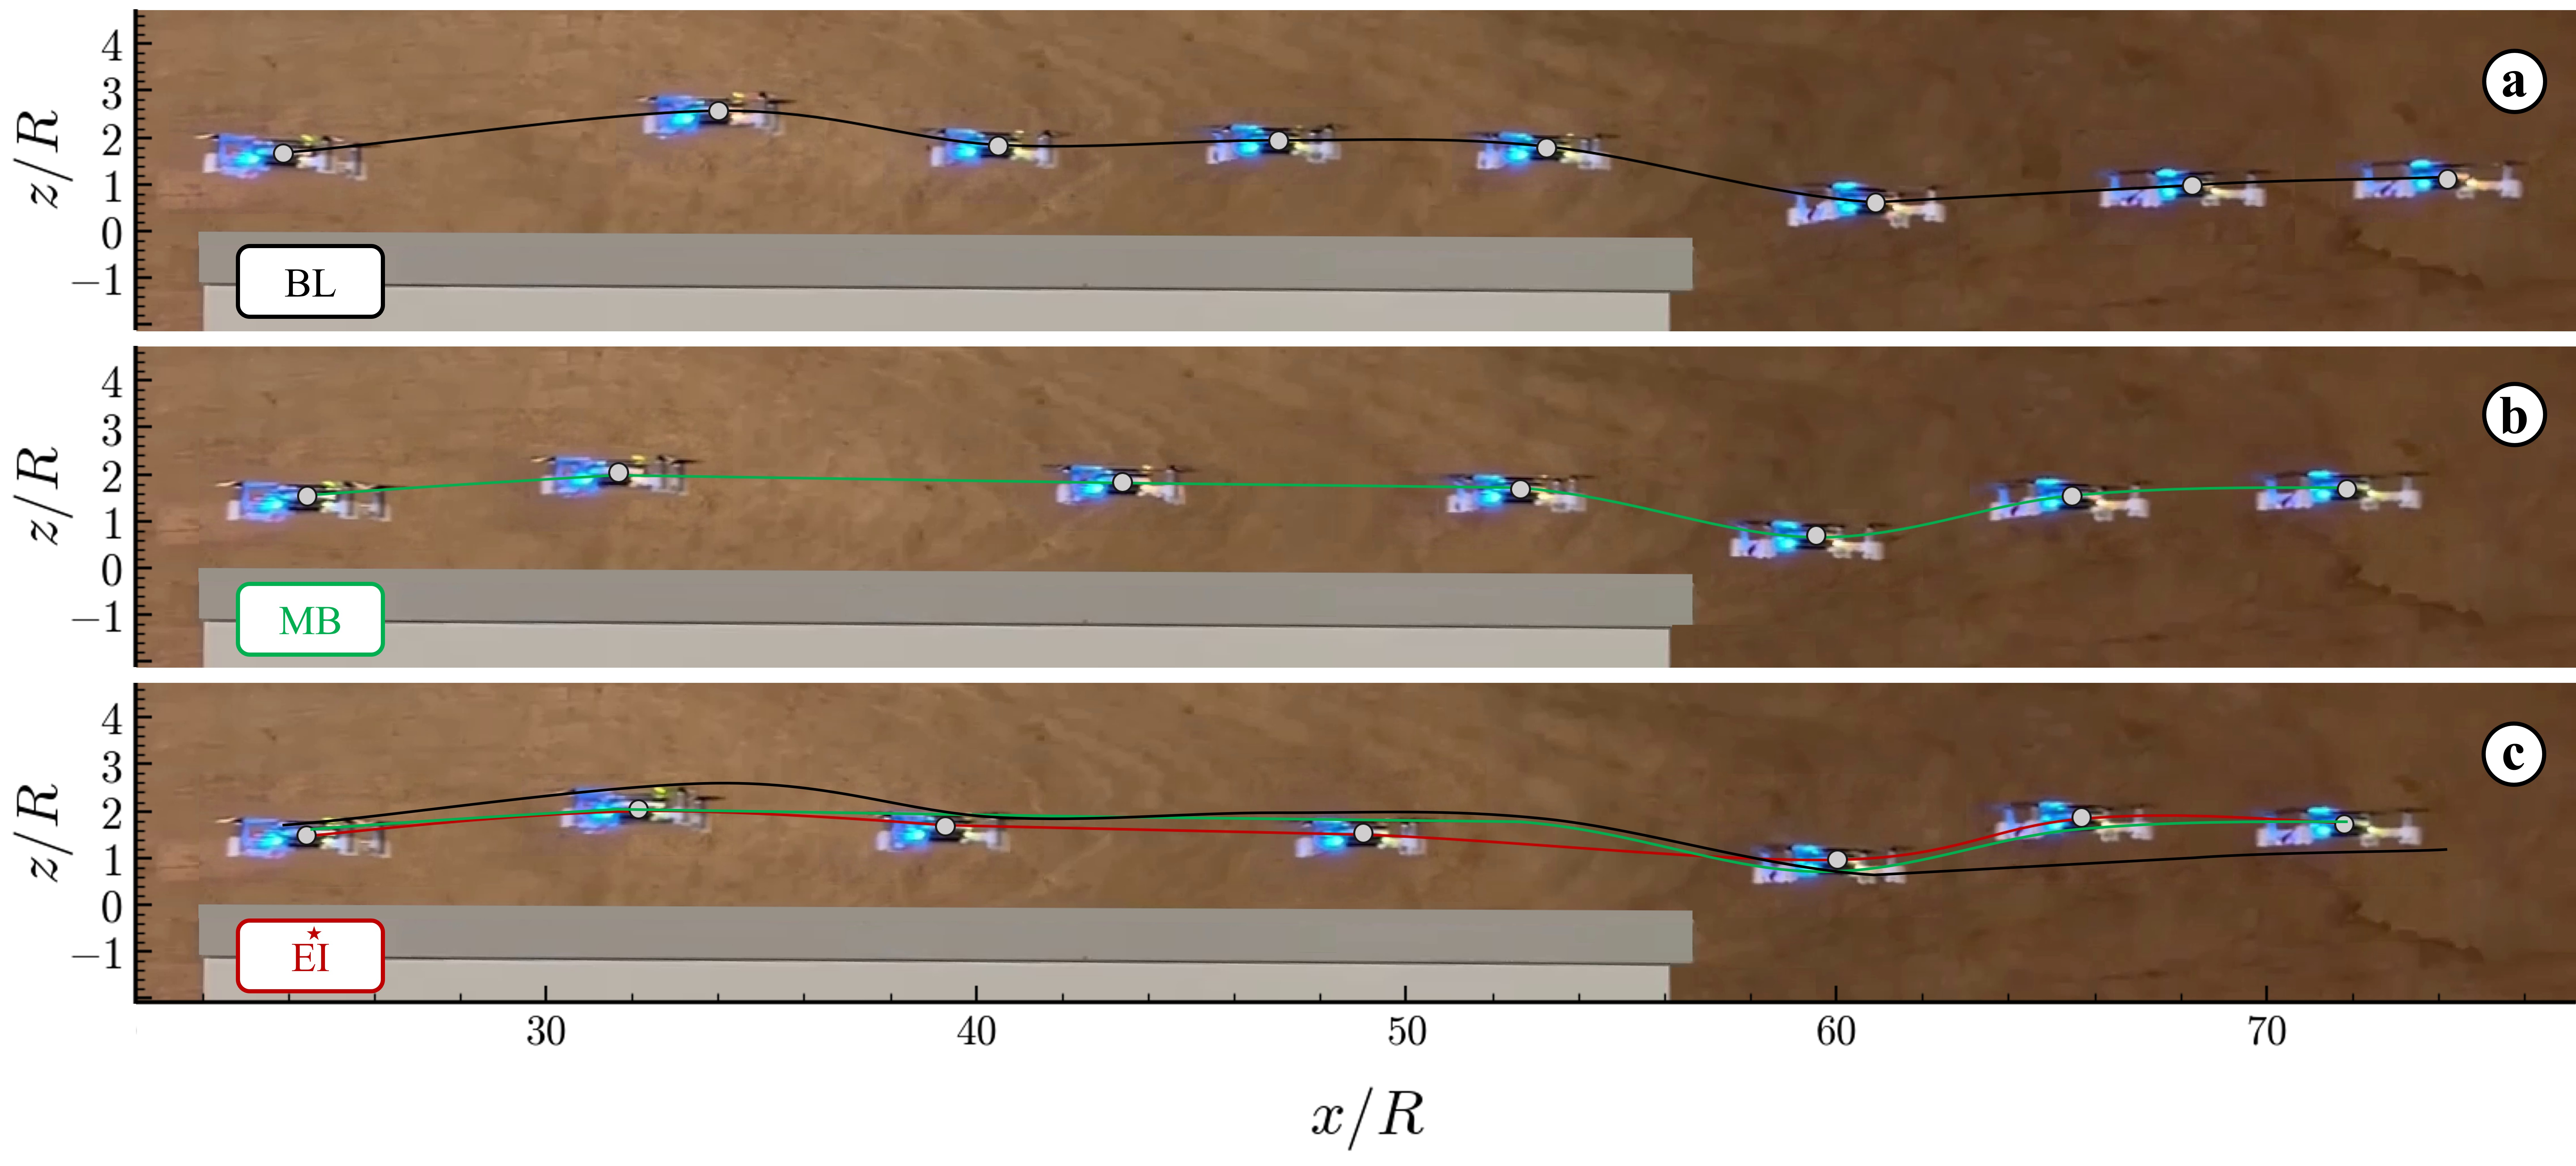
\includegraphics[width=\textwidth]{Results/Real_comparison.jpg}
\caption{Video-frame comparison of representative nominal-condition flights: (a) baseline policy $\pi_{\mathrm{BL}}$, (b) model-based policy $\pi_{\mathrm{MB}}$, and (c) best Expected-Improvement policy $\pi_{\mathrm{EI}}^{\star}$. The overlaid curves trace the measured vehicle path.}
\label{fig:real-comparison}
\end{figure*}

\subsection{Generalization Across Operating Conditions}
\label{sec:results-generalization}

Up to this point, the reward-transfer surrogate has been calibrated at the single nominal operating condition $(z^\ast/R,\,v_x^\ast/v_h)=(1.5,0.079)$. At this condition, the model-based policy produced a clear improvement over the baseline policy, and only a few additional physical evaluations were required for the GP discrepancy $\delta$ to capture part of the residual mismatch between the DT and physical rewards. Expected Improvement could consequently identify a policy with substantially better physical performance even though its DT reward was only marginally higher than that of $\pi_{\mathrm{MB}}$. The final campaign block investigates whether this policy correction remains useful when both the desired clearance and the forward velocity are changed.

Two additional operating conditions are considered: a low-speed, larger-clearance crossing at $(z^\ast/R,\,v_x^\ast/v_h)=(2.5,0.045)$ and a higher-speed, small-clearance crossing at $(1,0.113)$. The trajectory comparisons are reported in Fig.~\ref{fig:generalization-trajectories}. At each condition, the built-in PID controller executes the condition-specific baseline policy $\pi_{\mathrm{BL}}$, while a new model-based policy is computed using the same frozen parameter vector $\widehat{\boldsymbol{\theta}}_p$ identified at the end of the information phase. The nominal best correction is then transferred by applying the same three coefficients $\mathbf a=[a_A,a_B,a_C]^\top$ relative to the condition-specific model-based policy. This scaling preserves the learned correction structure without imposing the nominal reference correction as a fixed altitude offset.

In both operating conditions, the condition-specific model-based policy markedly improves tracking relative to the corresponding baseline policy. At $(z^\ast/R,\,v_x^\ast/v_h)=(2.5,0.045)$, the transferred policy provides a further, albeit modest, improvement. At the higher-speed, small-clearance condition $(1,0.113)$, however, its physical reward is slightly lower than that of the model-based policy. This loss is important: the transferred correction was learned from discrepancies measured only at the nominal condition $(1.5,0.079)$, whereas the relative importance of the unmodeled transients changes with velocity, clearance, and the magnitude of the model-based action. Transfer therefore provides an informed initialization, but it does not replace condition-specific learning when the operating condition moves away from the region represented in the reward-transfer surrogate dataset.

\begin{figure}[t]
\centering
\resultfigure{Results/stage_6_generalization_trajectory_comparison.pdf}
\caption{Generalization at (a) $(z^\ast/R,\,v_x^\ast/v_h)=(2.5,0.045)$ and (b) $(1,0.113)$: PID, local model-based, transferred RT, and condition-specific EI policies.}
\label{fig:generalization-trajectories}
\end{figure}

A direct comparison of rewards across these missions requires the different baseline difficulty to be removed. The DT and physical quantities are therefore normalized independently by their condition-specific baseline-policy values according to Eq.~\eqref{eq:normalized-score}. The DT and physical scores are denoted by $\mathcal S_{\circ}$ and $\mathcal S_{\bullet}$, respectively. By construction, $\mathcal S_e=0$ for the corresponding baseline policy and a larger value indicates a greater reduction of the tracking cost. This normalization places missions with different velocities and clearances on the same improvement scale and defines the normalized reward-transfer surrogate used across operating conditions.

In this more general formulation, the GP discrepancy depends on both the policy and the operating condition,
\begin{equation}
 \widehat{\mathcal S}_{\bullet}=
 \widehat{\mathcal S}_{\bullet,\mathrm{aff}}(\mathcal S_{\circ})+
 \widehat{\delta}\!\left(\mathbf a,z^\ast/R,v_x^\ast/v_h\right).
 \label{eq:generalized-surrogate}
\end{equation}
The vector $\mathbf a$ contains the three coefficients that modify the condition-specific model-based policy, while $(z^\ast/R,\,v_x^\ast/v_h)$ identifies the operating condition. Additional experiments distributed over the domain of interest would therefore train the normalized reward-transfer surrogate to propose a condition-specific correction instead of reproducing the same transferred policy everywhere. The present experiments provide an initial demonstration of this extension rather than a complete mapping of the velocity-clearance domain.

The normalized physical score is compared with its DT counterpart in Fig.~\ref{fig:generalization-reward}. Black markers correspond to $(z^\ast/R,\,v_x^\ast/v_h)=(1.5,0.079)$, orange markers to $(2.5,0.045)$, and purple markers to $(1,0.113)$. The transferred-policy diamond improves slightly on the model-based-policy square at the low-speed, larger-clearance condition. At the higher-speed, small-clearance condition, the ordering is reversed and the transferred policy performs slightly worse than $\pi_{\mathrm{MB}}$. A correction calibrated at one operating condition therefore cannot be assumed to retain the same ranking elsewhere, which motivates extending the surrogate across the operating domain rather than relying on direct policy transfer alone.

\begin{figure}[t]
\centering
\resultfigure{Results/stage_6_PID_normalized_reward_generalization.pdf}
\caption{Normalized reward-transfer surrogate across the nominal and two additional operating conditions.}
\label{fig:generalization-reward}
\end{figure}

The higher-speed, small-clearance condition is therefore used to demonstrate how the normalized reward-transfer surrogate can be extended locally. Two EI-guided physical evaluations are added at $(z^\ast/R,\,v_x^\ast/v_h)=(1,0.113)$. The first explores an uncertain policy direction and performs poorly, yielding approximately $\mathcal S_{\bullet}=0.57$, as indicated by the small purple marker in Fig.~\ref{fig:generalization-reward}. Once this observation updates the condition-aware GP discrepancy, the second evaluation reaches a new condition-specific best of approximately $\mathcal S_{\bullet}=0.83$, marked by the purple star, and exceeds the corresponding model-based policy. Its policy and physical trajectory are included in Fig.~\ref{fig:generalization-trajectories}(b). Unlike the nominal transferred correction, this policy remains closer to $\pi_{\mathrm{MB}}$, suggesting that the model-based policy was already near a favorable local optimum at the smaller clearance and higher velocity.

Only two condition-specific EI iterations are used here, so the result is interpreted as a proof-of-concept local extension of the RT workflow rather than as convergence of a general surrogate. At a new operating condition, the local DT first supplies a model-based policy that already improves substantially over the baseline policy. When direct transfer fails to improve that policy, a small number of physical interactions can reveal how the GP discrepancy has changed and redirect the search toward a better condition-specific solution. Repeating this process over the velocity-clearance domain would progressively calibrate $\widehat{\delta}(\mathbf a,z^\ast/R,v_x^\ast/v_h)$ and enable the generation of policies tailored to the requested operating condition while retaining the model-based policy as the safe and data-efficient reference.

\section{Conclusions and Outlook}
\label{sec:conclusion}

This work demonstrated Reinforcement Twinning for predictive trajectory control of a micro aerial vehicle crossing a finite obstacle in ground effect. The information phase provided evidence that the designed experiments added more than visual diversity: the cumulative smallest Fisher eigenvalue grew much faster than for repeated baseline experiments, and restricting the design from the broad domain to the near-wall domain restored information gain as the former began to saturate. Although the identified model parameters remained correlated, the resulting ground-effect function was well constrained over the control-relevant clearance range. Parameter decorrelation was therefore not treated as the objective by itself; the relevant outcome was the improved identification of the weakest observable parameter direction and of the aerodynamic correction used by the controller.

Model-based optimization remained the backbone of the framework. The identified DT generated an anticipatory model-based policy that improved tracking without replacing the onboard feedback controller and while satisfying the adopted virtual safety constraints. The remaining replay error then motivated the performance phase rather than invalidating the DT. Fractional and Sobol policies calibrated the reward-transfer surrogate, while Expected Improvement directed subsequent physical experiments toward uncertain and potentially better policies. With few additional interactions, the resulting $\pi_{\mathrm{EI}}^{\star}$ outperformed the model-based policy by compensating for response features that the low-order static model could not rank accurately. In this way, the DT restricted the search to a screened, high-performing neighborhood, and physical rewards were used specifically to learn the GP discrepancy within that neighborhood.

The off-nominal experiments clarified both the potential and the present limits of generalization. Directly transferring the nominal correction produced a modest gain at one operating condition but slightly underperformed the corresponding model-based policy at the other. After two condition-specific EI evaluations, the normalized reward-transfer surrogate identified an improved local policy. This result supports the data efficiency of local refinement, but it does not establish a surrogate that is converged over a continuous velocity-clearance domain.

The conclusions are therefore limited to the tested envelope. The ground-effect model represents an unsteady rotor-surface interaction with a static two-parameter law and cannot reproduce every transient feature. The physical experiments were constrained to $z/R\geq0.5$, so the results do not support extrapolation toward contact, and generalization was examined at only two additional operating conditions. Future work should extend the campaign across a denser velocity-clearance domain, account explicitly for repeated-measurement uncertainty in the reward-transfer surrogate, and investigate richer unsteady aerodynamic models, moving landing surfaces, and onboard or real-time policy adaptation. Within the present limits, the campaign shows how RT can combine interpretable physics, virtual safety screening, and a targeted data-driven correction to improve control performance without requiring unconstrained model-free exploration.

\section*{Acknowledgment}
The authors gratefully acknowledge the technical support of the von Karman Institute for Fluid Dynamics.

\bibliographystyle{IEEEtran}
\bibliography{references}

\end{document}



